\documentclass[12pt,a4paper]{article}

\usepackage[T1,T2A]{fontenc}
\usepackage[utf8]{inputenc}
\usepackage[russian, english]{babel}
\usepackage{amsmath, amssymb, mathtools}
\usepackage[top=1in, bottom=1in, left=0.7in, right=0.7in]{geometry}
\usepackage{microtype}
\usepackage{indentfirst}
\usepackage{setspace}
\usepackage{enumitem}
\usepackage{booktabs}
\usepackage{float}
\usepackage{graphicx}
\usepackage{subcaption}
\usepackage{tabularx}
\usepackage[unicode=true, colorlinks=true, linkcolor=blue, urlcolor=blue, citecolor=blue]{hyperref}

\graphicspath{{../rl-credit-scoring-sim/outputs/}}
\setstretch{1.08}

\title{Controlled State-Dimensionality Study\\for Weekly Threshold Control in Credit Scoring}
\author{}
\date{}

\begin{document}
\selectlanguage{english}

\maketitle
\tableofcontents
\clearpage

\section{Introduction}

This report describes the current state of the repository after it was re-centered around a controlled state-dimensionality experiment for weekly threshold control in credit scoring. The project is not a generic benchmark on public tabular datasets and it is not a pointwise approval classifier. Its object of control is a portfolio policy. Each week the controller selects score cutoffs for new and repeat applicants, the simulator accepts all applications above those cutoffs, and the resulting cohort produces repayments, defaults, and late recoveries over future weeks. Because the timing of cash flows is delayed, portfolio quality cannot be evaluated from the current cohort alone. A policy that looks attractive on a one-week horizon can still produce a weaker end-of-episode portfolio once defaults and capital pressure materialize.

This distinction is the main reason the repository remains relevant as a research artifact. In real consumer lending, threshold design is often revised at a batch level rather than on every individual file. The operational question is therefore not only ``which applications are good today,'' but also ``which weekly score frontier keeps the portfolio profitable, solvent, and stable over time.'' The present simulator makes that temporal trade-off explicit. It models weekly application inflow, segment heterogeneity, delayed loss realization, partial recoveries, portfolio-level capital usage, and a reward function that combines profitability with risk and operational constraints.

The current repository focus is narrower and more controlled than the broader framework from which the project evolved. The central research question is now: \emph{how much does observation design matter when everything else in the threshold-control problem is held fixed?} To answer this, the implementation compares four observation sizes, namely 12, 20, 30, and 50 features, while keeping environment dynamics, reward design, warm-up logic, terminal settlement, seeds, scenarios, baselines, RL algorithms, and the train/evaluation protocol unchanged.

That controlled setup matters for interpretation. It allows the dimensionality result to be attributed to the information content and complexity of the state vector rather than to hidden changes in reward shaping, scenario difficulty, or comparison controllers. The main exported conclusion is not that reinforcement learning automatically dominates rule-based policies. In fact, the strongest overall controller in the quick-profile outputs remains a non-RL baseline. The more precise conclusion is that state design materially changes RL quality, that richer portfolio state helps up to a point, and that the gain is strongly algorithm-dependent.

The updated repository supports a richer thesis-style narrative than the previous compact note. The main contributions evidenced by the current code and outputs are the following.
\begin{itemize}[leftmargin=*]
    \item The simulator implements weekly portfolio control with delayed credit outcomes, delayed rewards, terminal settlement, and separate thresholds for new and repeat clients.
    \item The dimensionality experiment changes only \texttt{state\_dim}, which makes the 12D--20D--30D--50D comparison a controlled methodological study rather than a loose sequence of experiments.
    \item The exported tables show that the best RL frontier improves from 12D to 30D and then largely saturates from 30D to 50D.
    \item The same exports also show that additional dimensionality does not help all algorithms equally: DQN improves substantially, Double-DQN peaks earlier and collapses at 50D, PPO is effectively unchanged, and SAC remains unstable.
    \item Weekly reward maximization and raw profit maximization are not identical objectives in this repository. The results therefore reveal trade-offs among profitability, default rate, approval rate, capital usage, and volatility rather than a single scalar ranking only.
\end{itemize}

\section{Problem Framing and Research Motivation}

\subsection{Why weekly threshold control is the research object}

Many credit-scoring discussions are framed as one-shot classification problems: estimate default probability, choose a threshold, and accept or reject. That view is useful for static offline validation, but it misses the managerial reality that threshold decisions are often implemented at a portfolio level and revised periodically. A lender does not only care about cross-sectional predictive accuracy. It also cares about how this week's approval policy changes next month's outstanding balance, the realized default rate in the reward window, the available capital headroom, and the composition of new versus repeat borrowers.

The repository therefore treats the control variable as a weekly threshold policy. The agent does not see one application at a time and it does not make one-step approval decisions. Instead, it controls a score frontier for the next weekly batch. This is closer to a practical policy-management problem: the model must choose a weekly level of selectivity under uncertainty, then observe delayed consequences.

This framing has two academic advantages. First, it turns the problem into a genuine sequential decision process with delayed consequences. Second, it makes policy evaluation economically interpretable. A weekly threshold can be discussed in terms of profitability, capital usage, and realized defaults in a way that resembles portfolio management rather than abstract classification.

\subsection{Why delayed outcomes and delayed rewards matter}

The simulator explicitly separates origination from realization. When a loan is accepted in week $t$, the relevant cash flow does not necessarily arrive in week $t$. A performing loan produces payoff only after its duration elapses. A default creates a negative cash flow, and a recovered default creates a later positive recovery cash flow. As a result, the immediate quality of the current cohort is not a sufficient performance measure for the controller.

This is not a cosmetic modeling choice. It directly changes what ``good control'' means. A policy may accept a slightly riskier cohort today and appear to increase current approval or current expected profit, but after the delayed defaults arrive the total portfolio path can be worse. Conversely, a stricter policy can look locally conservative and temporarily underperform, yet generate a better end-of-horizon trajectory because later defaults are avoided and capital is preserved.

The repository keeps this logic in two different places. First, delayed outcomes are created in the simulator itself: accepted loans schedule future repayment, default-loss, and optional late-recovery events. Second, delayed reward is enabled in the active configuration, which means that the reward function uses realized portfolio cash flows instead of only the current cohort's expected profit. This is why the thesis interpretation must focus on full-trajectory portfolio quality rather than one-step cohort economics.

The diagnostic artifact \texttt{outputs/dim\_30/locally\_worse\_globally\_better.csv} makes the idea concrete. In the adverse-stress setting, several agents exhibit a negative early gap but a large positive final gap, meaning that short-run underperformance and long-run portfolio superiority can coexist. For example, the 30D DQN row records an early gap of approximately $-643.46$ and a final gap of approximately $250{,}578.20$ under the pipeline's diagnostic comparator. This does not prove that RL always wins under stress. It does show why delayed evaluation is essential: early and final rankings are not guaranteed to coincide.

\subsection{Why separate thresholds for new and repeat clients are essential}

The simulator distinguishes new and repeat applicants at the structural level. Their base score distributions, default-response functions, recovery probabilities, loan sizes, and durations differ. This distinction is economically plausible: repeat clients typically contain more behavioral information and often exhibit different risk-return characteristics from newly acquired borrowers.

Because of that structural asymmetry, a shared threshold can be suboptimal even when both segments are scored on the same nominal scale. The repository therefore treats split-policy control as the default design. The action is normally a pair of thresholds rather than a single cutoff, and the observation includes segmented approval and default indicators. The dedicated \texttt{split\_policy\_dynamics} scenario strengthens this point by making new clients deteriorate while repeat clients improve.

This split-policy logic is especially important for interpretation of dimensionality. A richer state is useful only if the additional coordinates capture economically meaningful asymmetry. Several of the 20D, 30D, and 50D additions do exactly that: they add segment shares, segment-specific expected default indicators, accepted-share ratios, and threshold-gap history. The experiment is therefore not about abstract dimensionality for its own sake, but about whether a richer description of segmented weekly portfolio state helps the controller.

\section{Reference Boundary and Current Repository Scope}

The folder \texttt{Optimizing-Acceptance-Threshold-in-Credit-Scoring-using-Reinforcement-Learning-master} remains a reference-only snapshot and is not the source of truth for the current report. According to \texttt{notes/reference\_study.md}, the following mechanics were retained from the earlier study: weekly interaction, threshold control, delayed outcomes, delayed rewards, warm-up logic, and scenario-based distribution shift. The active implementation extends that foundation in several directions that are essential for the present thesis interpretation.

\begin{itemize}[leftmargin=*]
    \item Split-policy control for new and repeat applicants is part of the main design rather than an edge case.
    \item The experiment runner is configuration-driven and supports a controlled comparison of observation sizes.
    \item Reward shaping includes explicit portfolio-level penalties for default rate, approval pressure, capital usage, and volatility.
    \item The controller set is broader: DQN, Double-DQN, PPO, and SAC are compared against several non-RL baselines.
    \item Evaluation is multi-scenario, multi-seed, and exported with bootstrap confidence intervals and figure-ready artifacts.
\end{itemize}

This boundary is important because the thesis text should not describe the project as if it still used the original one-dimensional state or a single shared threshold only. The current repository is a more elaborate simulation framework whose immediate empirical focus is the controlled dimensionality study.

\section{Environment and Portfolio Simulator}

\subsection{Episode timeline}

The current environment follows a three-stage timeline that is implemented explicitly in \texttt{src/rl\_credit\_scoring\_sim/env/simulator.py}.
\begin{enumerate}[leftmargin=*]
    \item \textbf{Warm-up phase.} The simulator runs 8 initial weeks with the default thresholds. These weeks populate outstanding loans, recent profit history, and rolling default information before the controller begins to act.
    \item \textbf{Interactive phase.} During the 26 interactive weeks of the quick profile, the controller chooses weekly thresholds and the simulator records the resulting approvals, expected cohort characteristics, realized portfolio cash flows, and reward components.
    \item \textbf{Terminal settlement.} When the interactive horizon ends, remaining pending interactive cash-flow events are settled so that the episode summary is not artificially truncated by loans whose repayment or recovery would have occurred after the last decision week.
\end{enumerate}

This terminal-settlement step is especially important. Without it, a controller that originates many longer-duration loans near the end of the episode would be penalized mechanically because their positive cash flows would fall outside the measured window. The current implementation adds both terminal profit and terminal NPV to the final week's realized values, which makes the episode summary more faithful to the actual portfolio consequences of the policy.

\subsection{Weekly simulation logic}

Each simulated week begins with a scenario-specific market state. The scenario defines how repeat share, score drift, default drift, noise level, recovery probability, loan amount multiplier, and shock timing evolve over the horizon. Given that market state, the simulator draws weekly volumes for new and repeat segments, generates score distributions for both segments, converts scores into default probabilities through segment-specific logistic response functions, samples repayment/default/recovery outcomes, and assigns loan principal and duration distributions.

The controller then supplies a pair of thresholds $(\tau^{new}_t, \tau^{repeat}_t)$. Every application with score above the relevant threshold is accepted. Accepted loans contribute immediately to the future event queue, not necessarily to current realized profit. The simulator records both expected current-cohort quantities and realized portfolio quantities. This separation matters:
\begin{itemize}[leftmargin=*]
    \item \texttt{expected\_profit\_current} and \texttt{expected\_npv\_current} summarize the newly accepted cohort under the current week's market conditions;
    \item \texttt{realized\_profit} and \texttt{realized\_npv} summarize the cash flows that actually arrive in the current week from loans originated earlier.
\end{itemize}

The episode summary exported to the main CSV files then aggregates realized interactive profit and realized NPV over the whole episode. The repository keeps the legacy column name \texttt{expected\_profit\_mean} in its exported summary tables, but the current \texttt{episode\_summary()} implementation computes this value from realized weekly profits plus terminal settlement. In the discussion below, the original column name is retained when citing output files, but substantively it should be read as realized final portfolio profit under the simulator.

\subsection{Scenario design}

The six active evaluation scenarios are loaded from \texttt{configs/scenarios.yaml}. They are not arbitrary labels. Each one stresses a specific weakness of a threshold policy and therefore provides a reasoned test bed for cross-controller interpretation.

\begin{table}[H]
    \centering
    \small
    \begin{tabularx}{0.98\textwidth}{p{0.20\textwidth}X}
        \toprule
        Scenario                         & Interpretation                                                                                                                                                                                                              \\
        \midrule
        \texttt{base\_market}            & Stable market with moderate approval and default dynamics. This scenario is the cleanest test of whether the controller can exploit signal without fighting strong regime shifts.                                           \\
        \texttt{drift}                   & Gradual deterioration in new-client scores, rising default pressure, mild volume growth, and a small negative recovery shift. This tests whether the controller reacts adequately to a slow but persistent quality decline. \\
        \texttt{adverse\_stress}         & Abrupt negative shock, stronger default increases, higher noise, and larger loan amounts. This scenario punishes excessive risk-taking and highlights the value of robust selectivity.                                      \\
        \texttt{class\_imbalance\_shift} & Growing new-client share combined with lower average new-client quality. This scenario rewards controllers that manage composition risk rather than only overall approval.                                                  \\
        \texttt{noise}                   & Stable mean structure with much noisier measurements and weekly application volume. This is a test of robustness against unstable observations and volume shocks.                                                           \\
        \texttt{split\_policy\_dynamics} & New clients deteriorate while repeat clients improve. This is the most direct test of whether a split threshold is useful and whether segmented state information is exploited well.                                        \\
        \bottomrule
    \end{tabularx}
    \caption{Scenario logic from \texttt{configs/scenarios.yaml}.}
    \label{tab:en-scenarios}
\end{table}

These scenarios are not only descriptive. They help explain why controller rankings differ. A myopic weekly profit-search baseline can dominate when the environment remains interpretable through current cohort economics, while a more state-aware RL controller can gain ground when segment asymmetry or stable market signal is exploitable. Under severe stress, however, strong risk control can matter more than flexible representation.

\section{Controlled Experimental Design}

\subsection{What is held fixed}

The present dimensionality experiment is intentionally controlled. The following elements remain constant across the 12D, 20D, 30D, and 50D runs.
\begin{itemize}[leftmargin=*]
    \item weekly simulator dynamics and the six-scenario evaluation suite;
    \item split-policy control semantics and the threshold grid from 35 to 85 with step 5;
    \item reward design, including delayed reward, risk-aware shaping, and constraint penalties;
    \item warm-up logic, interactive horizon, and terminal settlement;
    \item seeds 11, 23, and 37 in the active \texttt{quick} profile;
    \item training episodes, evaluation-run counts, and scenario randomization during training;
    \item the compared controller set: \texttt{dqn}, \texttt{double\_dqn}, \texttt{ppo}, \texttt{sac}, \texttt{static\_threshold}, \texttt{profit\_oriented}, \texttt{risk\_aware\_weekly}, \texttt{constraint\_aware\_weekly}, and \texttt{split\_policy\_static};
    \item the same bootstrap-CI machinery and the same output file structure.
\end{itemize}

The code even performs explicit repository-level validation to verify that the first 12 features are unchanged across every observation size, that controller coverage is complete, that required files exist, and that no future leakage is introduced by the added state coordinates.

\subsection{What changes}

The only experimental factor is the observation dimensionality:
\[
    \texttt{state\_dim} \in \{12, 20, 30, 50\}.
\]

The dimensionality comparison is therefore a study of state representation under constant environment and policy semantics. This is the correct framing for the thesis. The experiment is not testing different simulators, different rewards, or different datasets. It is testing whether additional state information improves the quality of threshold control and, if so, where the returns start to diminish.

\subsection{Observation layers}

The state space is expanded cumulatively.

\begin{table}[H]
    \centering
    \small
    \begin{tabularx}{0.98\textwidth}{p{0.11\textwidth}X}
        \toprule
        State size & Composition                                                                                                                                                                                                                                                                                                   \\
        \midrule
        12D        & Baseline state: week progress, overall and segment approval rates, rolling realized default rate, expected current default rate, realized profit, rolling profit volatility, projected capital usage, outstanding ratio, and normalized new/repeat thresholds.                                                \\
        20D        & 12D plus repeat-share, expected profit and expected NPV per application, realized NPV, weekly reward, threshold gap, capital headroom, and the gap between realized and expected default rate.                                                                                                                \\
        30D        & 20D plus lagged and rolling history: second-lag approval/default/profit/capital usage, four-week rolling approval/default/profit indicators, profit rolling standard deviation, and lagged threshold changes.                                                                                                 \\
        50D        & 30D plus richer segment and stability descriptors: segment-specific approval/default/profit signals, accepted-share ratios, rolling reward moments, cumulative reward and profit to date, capital-usage variability, outstanding-capital change, threshold-gap history, and current application-volume ratio. \\
        \bottomrule
    \end{tabularx}
    \caption{Cumulative observation construction. Exact ordered definitions are documented in \texttt{state\_dimension\_manifest.md}.}
    \label{tab:en-features}
\end{table}

This cumulative construction gives the state-size experiment a substantive interpretation.
\begin{itemize}[leftmargin=*]
    \item The 12D state is essentially a compact weekly dashboard: what just happened, how risky it looks, and what thresholds were used.
    \item The 20D state adds immediate economic context. It tells the controller not only what happened, but how much profit and NPV the last cohort implied and how much capital room remains.
    \item The 30D state adds memory. It allows the controller to compare the latest week with lagged and rolling history, which is especially relevant under drift and noisy volume.
    \item The 50D state adds greater segmentation and stability detail. It is the richest description, but also the most demanding one for optimization and generalization.
\end{itemize}

From a methodological perspective, the central hypothesis is that the 20D and 30D enrichments add signal that is genuinely useful for portfolio control, whereas 50D may start to add complexity faster than control value. The results support exactly that intermediate-saturation interpretation.

\section{Controllers}

\subsection{Rule-based and static baselines}

The baseline set is economically meaningful rather than decorative.
\begin{itemize}[leftmargin=*]
    \item \texttt{static\_threshold} applies one fixed shared threshold and therefore acts as the simplest non-adaptive benchmark.
    \item \texttt{split\_policy\_static} keeps different default thresholds for new and repeat clients but does not update them over time.
    \item \texttt{profit\_oriented} performs weekly grid search and selects the threshold pair with the highest current-cohort expected profit, deliberately ignoring broader portfolio constraints.
    \item \texttt{risk\_aware\_weekly} is a hand-crafted feedback controller that raises or lowers thresholds in response to rolling realized defaults, approval pressure, and capital usage.
    \item \texttt{constraint\_aware\_weekly} performs a weekly grid search with penalty-weighted violation terms, thereby operationalizing a more conservative multi-objective benchmark.
\end{itemize}

These baselines are important for interpretation because they span several distinct management styles: static, split-static, myopic profit chasing, hand-built reactive control, and explicit constraint-aware search. When RL loses to one of them, the thesis can say \emph{which kind of non-RL policy} remains competitive.

\subsection{RL agents}

The repository evaluates four RL algorithms.
\begin{itemize}[leftmargin=*]
    \item \texttt{dqn} and \texttt{double\_dqn} operate on the discrete threshold grid and are natural choices when weekly control is represented as selection from a finite action set.
    \item \texttt{ppo} and \texttt{sac} use continuous actions that are mapped back onto the same threshold range and rounded to the grid granularity.
\end{itemize}

This separation is analytically useful because it shows that dimensionality interacts with action representation. The current quick-profile results do not produce a single RL story. Instead, they show that value-based discrete controllers benefit much more from enriched state than the two continuous-policy agents do under the same budget.

\section{Reward Formulation and Metric Design}

\subsection{Reward function}

The reward mechanism is implemented in \texttt{src/rl\_credit\_scoring\_sim/env/reward.py}. With delayed reward enabled, the main terms are based on realized portfolio profit and realized NPV rather than only the current cohort's expectation. In simplified form, the weekly reward can be written as
\begin{equation}
    \label{eq:reward}
    \begin{aligned}
        r_t ={} & w_p \cdot \Pi^{realized}_t + w_n \cdot \mathrm{NPV}^{realized}_t - w_s \cdot \hat d_t \cdot 100 \\
                & - \lambda_d \bigl[\max(0, \bar d_t - 0.12)\bigr]^2 \cdot 1000                                   \\
                & - \lambda_a \left|\alpha_t - 0.42\right| \cdot 1000                                             \\
                & - \lambda_c \bigl[\max(0, c_t - 0.82)\bigr]^2 \cdot 1000                                        \\
                & - \lambda_v \max\!\left(0, \frac{\sigma_{\Pi,t} - 8500}{8500}\right) \cdot 1000,
    \end{aligned}
\end{equation}
where the active configuration sets $w_p = 1.0$, $w_n = 0.25$, $w_s = 0.35$, $\lambda_d = 9.0$, $\lambda_a = 2.0$, $\lambda_c = 3.5$, and $\lambda_v = 1.4$.

The reward is therefore intentionally multi-objective. It does not rank policies by raw profit alone. It rewards realized portfolio payoff, values discounted cash flow, discourages high expected default on the current accepted cohort, penalizes excess realized default in the rolling reward window, penalizes large deviations from the approval target, penalizes excessive projected capital usage, and penalizes excessive realized-profit volatility.

\subsection{Why this trade-off matters}

The reported results make little sense if the reader interprets them as a pure-profit contest. The repository's official selection rule for the best controller is: highest \texttt{cumulative\_reward\_mean}, then highest \texttt{expected\_profit\_mean}, then highest \texttt{stability\_index\_mean}, then lowest \texttt{default\_rate\_mean}. Consequently, a controller may produce slightly higher raw profit in one scenario and still lose on the main ranking if it does so with more volatility, stronger capital pressure, or more undesirable approval behavior.

The \texttt{noise} scenario is the clearest example. Across dimensions, \texttt{risk\_aware\_weekly} has the highest scenario-level profit by the repository's \texttt{expected\_profit\_mean} column, reaching $97{,}377.95$ in that scenario. Yet the reward-based scenario winner remains \texttt{profit\_oriented}, whose lower raw profit of $94{,}589.22$ is offset by better total reward under the implemented weighting and penalty structure. This is not a contradiction; it is exactly what a shaped portfolio reward is supposed to reveal.

\subsection{Reported metrics}

The core metrics used throughout the outputs are:
\begin{itemize}[leftmargin=*]
    \item approval rate;
    \item realized default rate;
    \item final portfolio profit (exported under the legacy name \texttt{expected\_profit\_mean});
    \item realized portfolio NPV;
    \item cumulative shaped reward;
    \item mean projected capital usage ratio;
    \item reward volatility;
    \item stability index, defined in code as $1 / (1 + \mathrm{reward\_volatility})$;
    \item threshold volatility, defined as the standard deviation of week-to-week threshold changes inside an episode.
\end{itemize}

Note that threshold volatility measures within-episode movement, not cross-seed variation in the chosen threshold level. This distinction becomes important when interpreting the best RL runs, because the exported winners are usually static within an episode even though different seeds may settle on different threshold pairs.

\section{Experimental Protocol}

The main thesis evidence comes from the active \texttt{quick} profile. The merged configuration loaded by the code corresponds to:
\begin{itemize}[leftmargin=*]
    \item 8 warm-up weeks and 26 interactive weeks;
    \item 260 configured applications per week before scale factors;
    \item training scale $0.80$, validation scale $0.90$, and test scale $1.00$ with \texttt{test\_subset\_fraction} $= 0.65$;
    \item 12 training episodes per RL seed;
    \item 4 evaluation runs per seed and scenario;
    \item seeds 11, 23, and 37;
    \item bootstrap confidence intervals at the 95\% level with 120 resamples in the active fast-CI mode because \texttt{full\_ci = false}.
\end{itemize}

The outputs are organized as follows.
\begin{itemize}[leftmargin=*]
    \item One directory per observation size: \texttt{outputs/dim\_12/}, \texttt{outputs/dim\_20/}, \texttt{outputs/dim\_30/}, and \texttt{outputs/dim\_50/}.
    \item Root-level cross-dimension summaries: \texttt{outputs/dimension\_comparison\_summary.csv}, \texttt{outputs/best\_rl\_by\_dimension.csv}, \texttt{outputs/overall\_best\_by\_dimension.csv}, and the \texttt{metric\_vs\_dimension\_*.png} figures.
\end{itemize}

The controlled-protocol validation is one of the stronger aspects of the current repository state. The dimensionality pipeline checks that:
\begin{itemize}[leftmargin=*]
    \item the first 12 features are unchanged across all dimensions under a common reset and fixed action sequence;
    \item seeds, scenarios, reward settings, and controller sets match across dimensions;
    \item the added features use only interactive history, last-week metrics, week index, and fixed configuration values;
    \item every controller finishes the expected number of runs in every dimension;
    \item all required CSV and plot artifacts exist and are non-empty;
    \item the best-row extracts are consistent with the global comparison summary.
\end{itemize}

This validity layer is valuable for the thesis because it supports the claim that the reported saturation pattern is not an artifact of silent protocol drift.

\section{Main Results}

\subsection{Best overall controller by dimension}

Table \ref{tab:en-best-overall} reports the strongest controller when baselines and RL agents are pooled together under the repository's official reward-based ranking rule.

\begin{table}[H]
    \centering
    \small
    \begin{tabular}{l l l r r r}
        \toprule
        State dim & Best overall              & Type     & Profit     & Reward     & Default rate \\
        \midrule
        12        & \texttt{profit\_oriented} & baseline & 76\,022.08 & 88\,080.60 & 0.1169       \\
        20        & \texttt{profit\_oriented} & baseline & 76\,022.08 & 88\,080.60 & 0.1169       \\
        30        & \texttt{profit\_oriented} & baseline & 76\,022.08 & 88\,080.60 & 0.1169       \\
        50        & \texttt{profit\_oriented} & baseline & 76\,022.08 & 88\,080.60 & 0.1169       \\
        \bottomrule
    \end{tabular}
    \caption{Best overall controller by dimension from \texttt{outputs/overall\_best\_by\_dimension.csv}.}
    \label{tab:en-best-overall}
\end{table}

Three points are important here. First, the flat baseline line across dimensions confirms that the experiment is truly isolating the effect of observation size on RL controllers rather than on the comparison set. Second, the leading baseline is not overwhelmingly better than every other non-RL policy. The runner-up \texttt{constraint\_aware\_weekly} achieves cumulative reward $88{,}000.75$, only about $79.85$ below \texttt{profit\_oriented}. Third, this means the top of the leaderboard is dominated by strong rule-based benchmarks, not by a trivial static threshold.

In substantive terms, the best overall result says that the current quick-profile environment still rewards well-designed weekly rule search. RL narrows the gap as the state becomes richer, but the repository does not support the stronger claim that RL already dominates policy search under all tested conditions.

\subsection{Best RL controller by dimension}

\begin{table}[H]
    \centering
    \small
    \begin{tabular}{l l r r r r r}
        \toprule
        State dim & Best RL              & Profit     & NPV        & Reward     & Approval rate & Capital usage \\
        \midrule
        12        & \texttt{dqn}         & 59\,197.47 & 57\,144.61 & 67\,308.36 & 0.4159        & 0.4454        \\
        20        & \texttt{double\_dqn} & 61\,096.44 & 58\,978.98 & 69\,812.02 & 0.4329        & 0.4569        \\
        30        & \texttt{dqn}         & 66\,758.29 & 64\,755.07 & 78\,219.69 & 0.3527        & 0.3902        \\
        50        & \texttt{dqn}         & 66\,946.81 & 64\,815.05 & 78\,198.39 & 0.3935        & 0.4280        \\
        \bottomrule
    \end{tabular}
    \caption{Best RL controller by dimension from \texttt{outputs/best\_rl\_by\_dimension.csv}.}
    \label{tab:en-best-rl}
\end{table}

Table \ref{tab:en-best-rl} gives the main empirical pattern of the study.
\begin{enumerate}[leftmargin=*]
    \item The move from 12D to 20D helps modestly. The best RL profit rises from $59{,}197.47$ to $61{,}096.44$, and cumulative reward rises from $67{,}308.36$ to $69{,}812.02$.
    \item The move from 20D to 30D is the decisive improvement. Profit increases by about $5{,}661.85$, NPV increases by about $5{,}776.10$, cumulative reward increases by about $8{,}407.67$, while default rate declines from $0.1260$ to $0.1185$.
    \item The move from 30D to 50D yields almost no additional reward. Profit improves by only about $188.53$, cumulative reward is slightly lower, and both approval rate and capital usage rise again.
\end{enumerate}

This pattern is exactly what a saturation story looks like. The 20D and 30D states add information that can be monetized into better control. The 50D state does not extend that gain in a comparable way.

The 30D row is especially interesting because it improves reward while becoming \emph{more selective}. Approval rate falls to $0.3527$ and capital usage falls to $0.3902$. This is not a reward gain caused by simply approving more loans. It is a gain produced by accepting a cleaner and more capital-efficient portfolio mix. That strengthens the interpretation that the additional lagged and rolling state variables are economically useful rather than merely descriptive.

\subsection{Algorithm-specific interaction with dimensionality}

The aggregate best-RL frontier hides important heterogeneity across algorithms. Table \ref{tab:en-rl-all} reports all four RL agents.

\begin{table}[H]
    \centering
    \small
    \begin{tabular}{l l r r r r}
        \toprule
        Agent                & State dim & Profit      & Reward       & Default rate & Threshold volatility \\
        \midrule
        \texttt{dqn}         & 12        & 59\,197.47  & 67\,308.36   & 0.1233       & 0.0000               \\
        \texttt{dqn}         & 20        & -15\,413.93 & -34\,719.92  & 0.1545       & 0.0000               \\
        \texttt{dqn}         & 30        & 66\,758.29  & 78\,219.69   & 0.1185       & 0.0000               \\
        \texttt{dqn}         & 50        & 66\,946.81  & 78\,198.39   & 0.1195       & 0.0000               \\
        \midrule
        \texttt{double\_dqn} & 12        & 59\,221.98  & 66\,915.54   & 0.1223       & 0.0000               \\
        \texttt{double\_dqn} & 20        & 61\,096.44  & 69\,812.02   & 0.1260       & 0.0000               \\
        \texttt{double\_dqn} & 30        & 57\,467.87  & 65\,247.13   & 0.1282       & 0.0000               \\
        \texttt{double\_dqn} & 50        & -49\,782.91 & -79\,329.16  & 0.1574       & 0.0000               \\
        \midrule
        \texttt{ppo}         & 12--50    & 12\,196.74  & 4\,958.59    & 0.1537       & 0.0000               \\
        \texttt{sac}         & 12        & -36\,379.87 & -57\,961.65  & 0.1674       & 3.0132               \\
        \texttt{sac}         & 20        & -22\,232.63 & -35\,997.61  & 0.1494       & 2.2454               \\
        \texttt{sac}         & 30        & -11\,904.25 & -26\,218.31  & 0.1535       & 2.6183               \\
        \texttt{sac}         & 50        & -72\,433.15 & -105\,961.13 & 0.1677       & 1.9269               \\
        \bottomrule
    \end{tabular}
    \caption{All RL agents across dimensions from the per-dimension \texttt{main\_overall\_summary.csv} files.}
    \label{tab:en-rl-all}
\end{table}

The algorithm-specific picture matters as much as the best-RL picture.
\begin{itemize}[leftmargin=*]
    \item DQN is highly sensitive to representation quality. It performs well at 12D, fails badly at 20D, then becomes the best RL controller by a wide margin at 30D and stays there at 50D.
    \item Double-DQN peaks earlier. It is the best RL method at 20D, remains competitive at 30D, and then collapses at 50D.
    \item PPO is numerically identical across all four dimensions down to the exported summary precision. Under the current quick-profile training budget, richer state does not change its learned outcome materially.
    \item SAC remains negative in every dimension and becomes especially poor at 50D.
\end{itemize}

This is strong evidence that dimensionality is not an isolated ``more is better'' dial. It interacts with optimization method and training budget. The added state dimensions are useful enough to improve the best RL frontier, but they do not produce universal improvement across all controllers.

\subsection{Cross-dimension figures}

\begin{figure}[H]
    \centering
    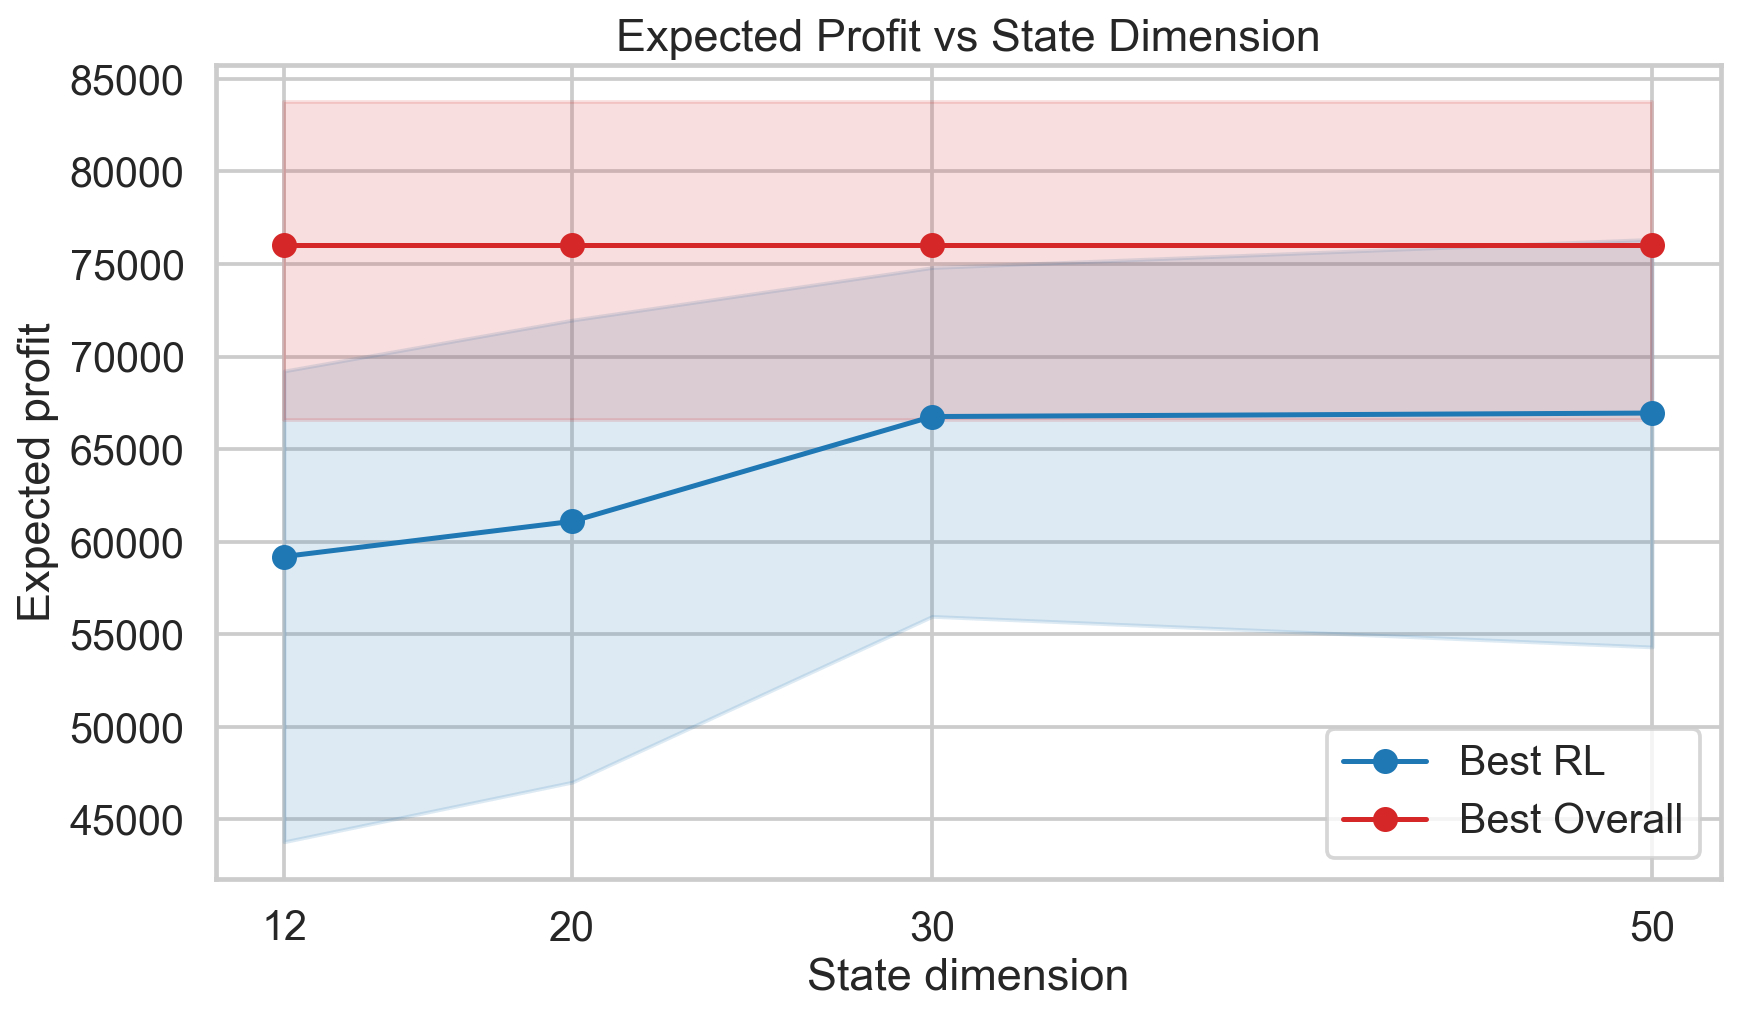
\includegraphics[width=0.82\textwidth]{metric_vs_dimension_expected_profit.png}
    \caption{Profit versus state dimension for the best RL controller and the best overall controller.}
    \label{fig:en-profit-vs-dim}
\end{figure}

\begin{figure}[H]
    \centering
    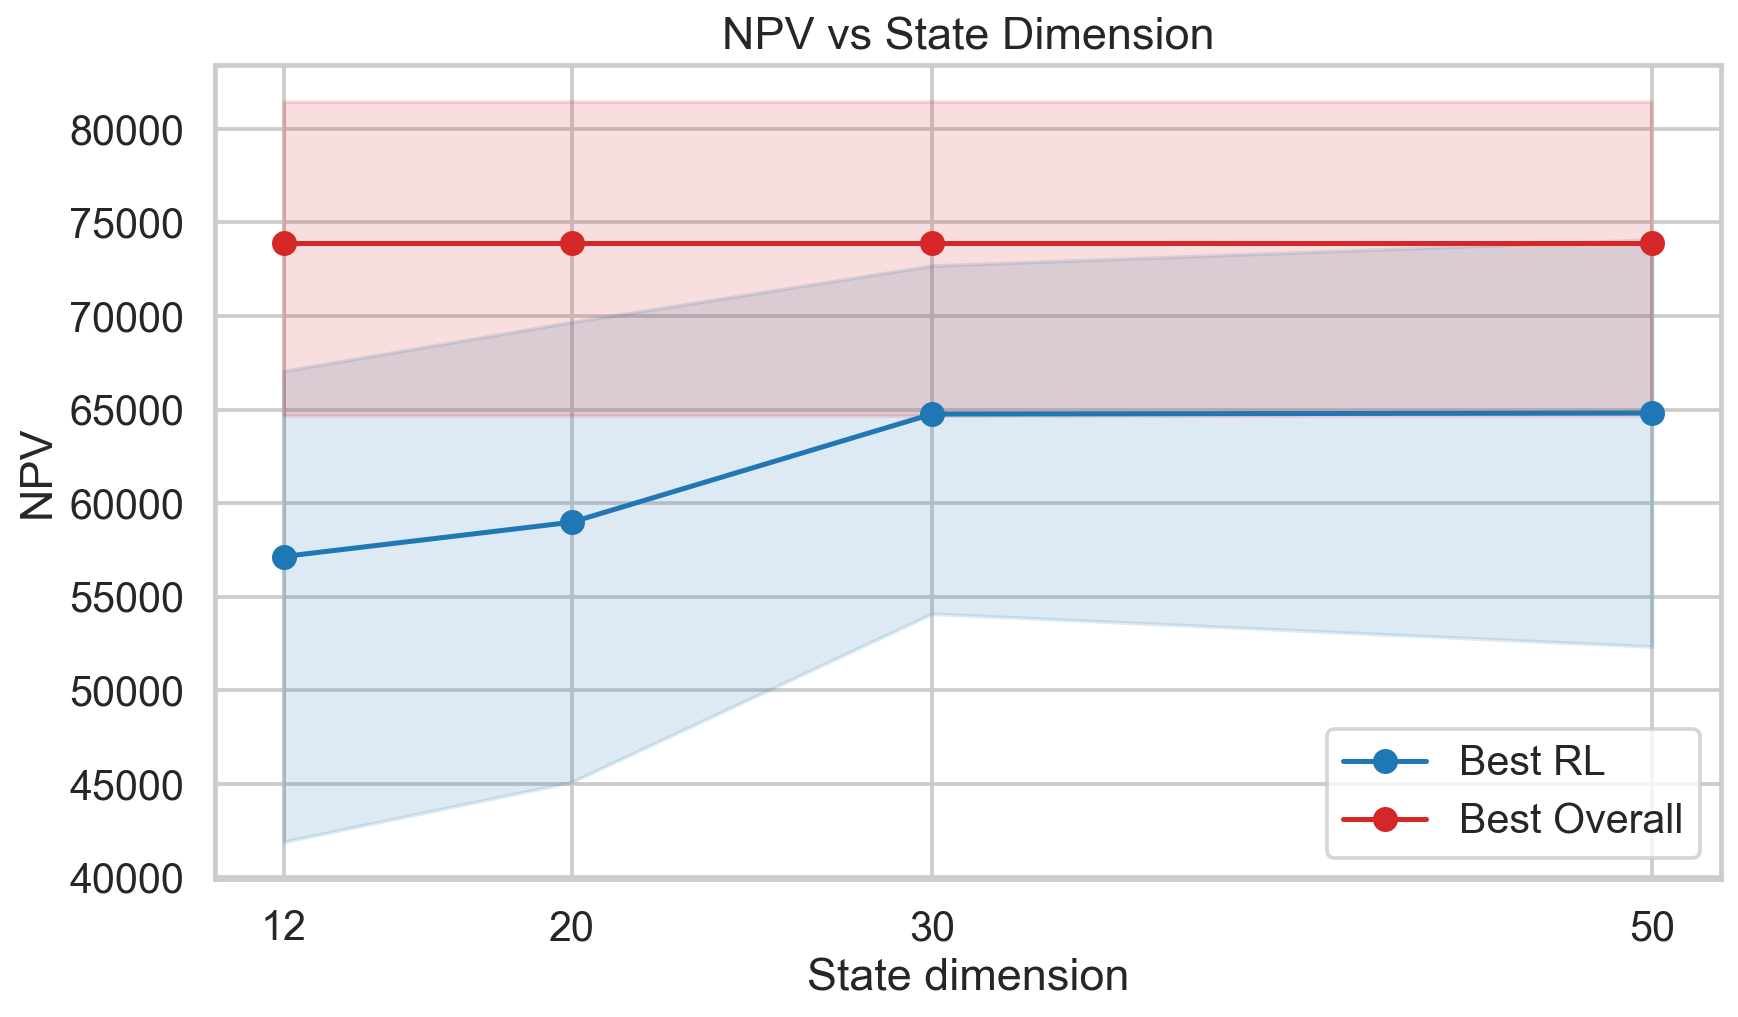
\includegraphics[width=0.82\textwidth]{metric_vs_dimension_npv.png}
    \caption{NPV versus state dimension.}
    \label{fig:en-npv-vs-dim}
\end{figure}

\begin{figure}[H]
    \centering
    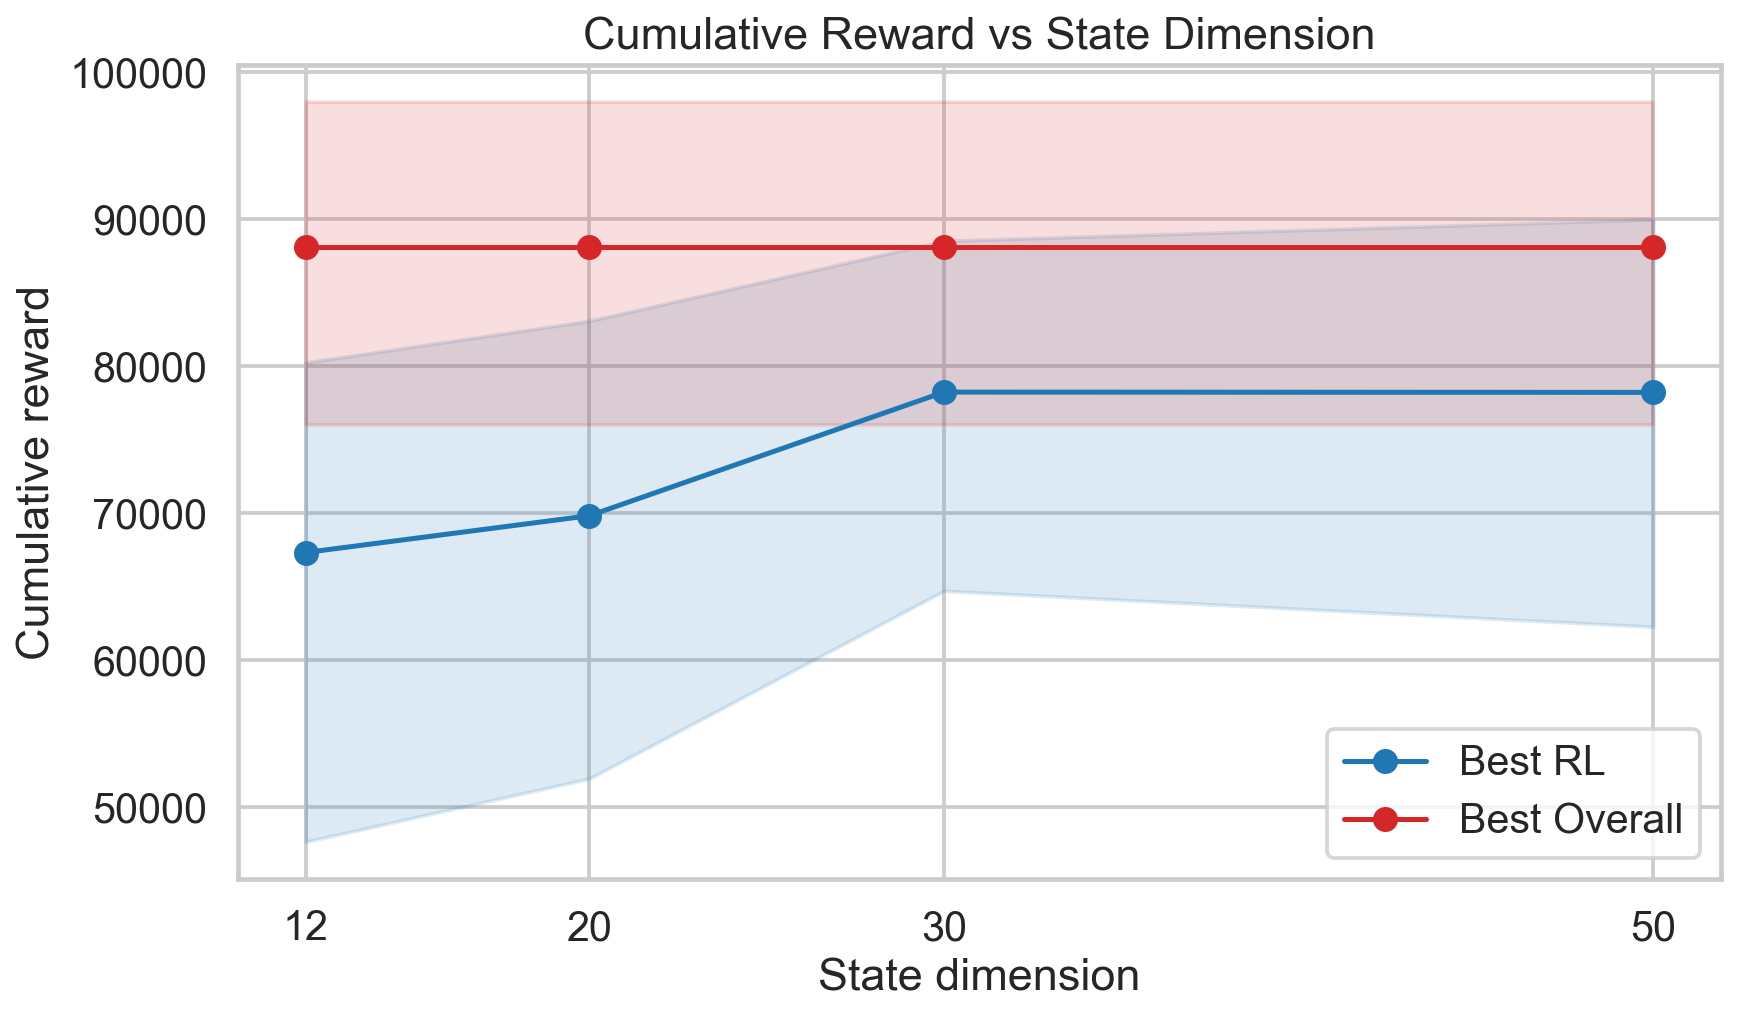
\includegraphics[width=0.82\textwidth]{metric_vs_dimension_cumulative_reward.png}
    \caption{Cumulative reward versus state dimension.}
    \label{fig:en-reward-vs-dim}
\end{figure}

\begin{figure}[H]
    \centering
    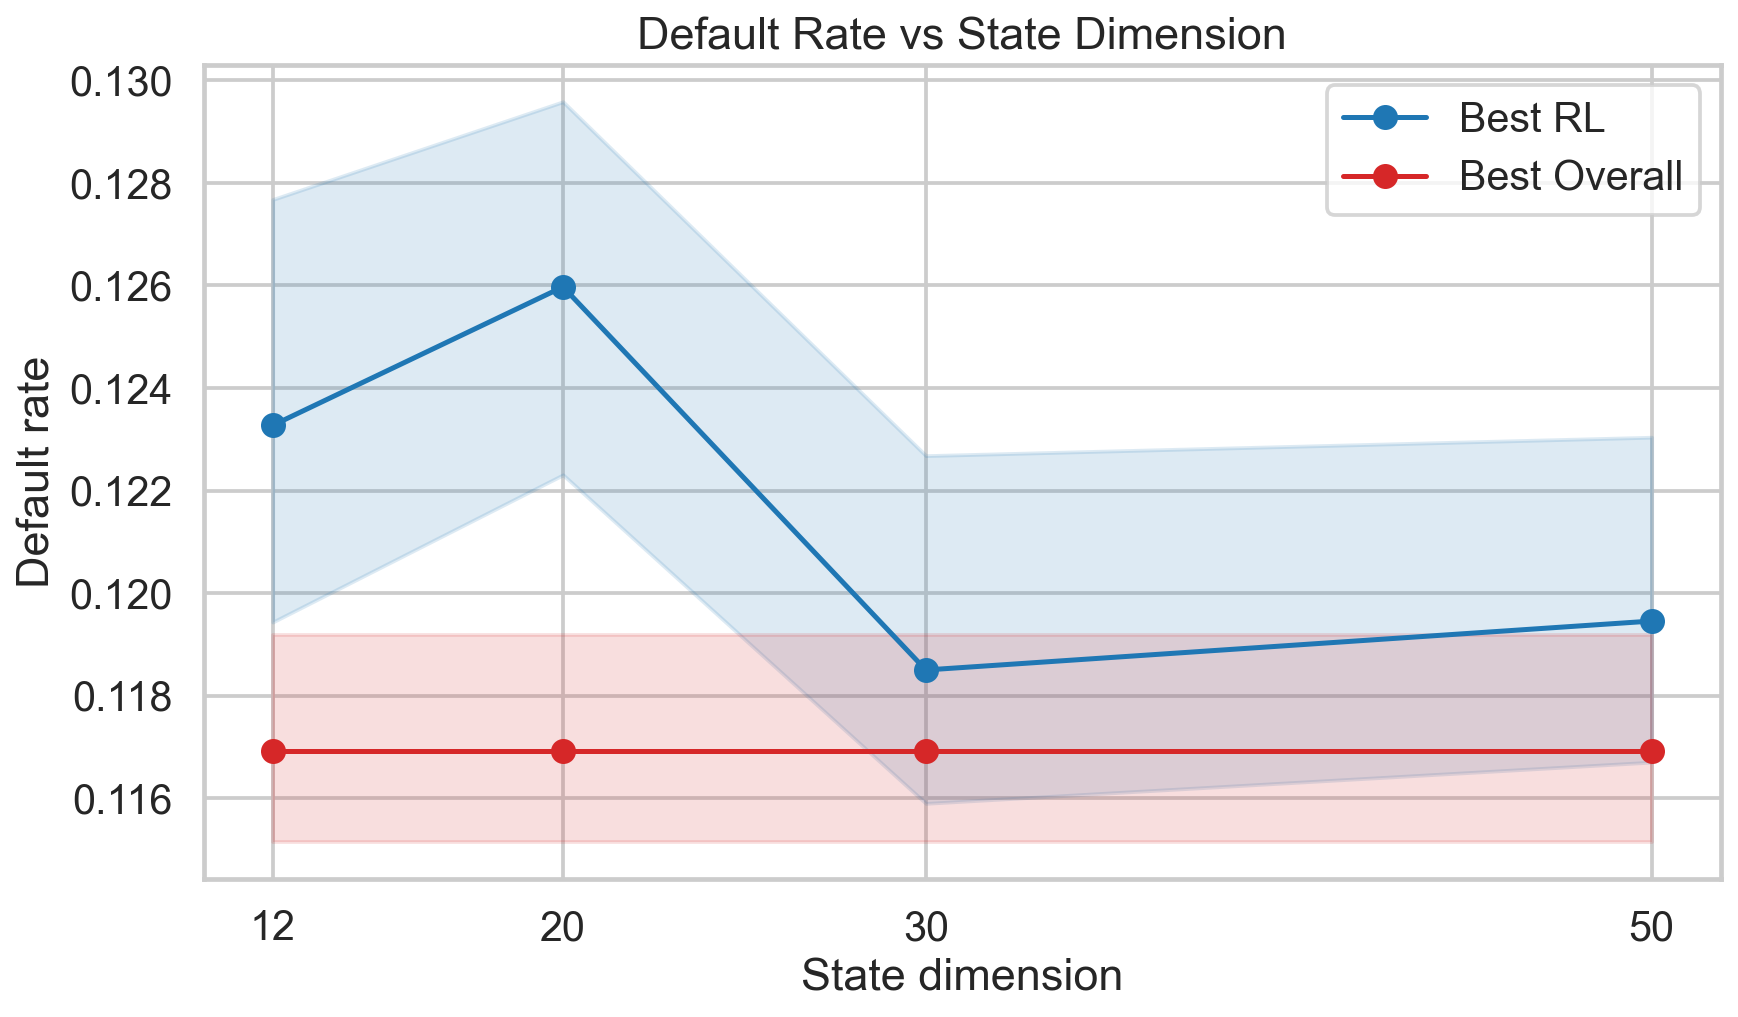
\includegraphics[width=0.82\textwidth]{metric_vs_dimension_default_rate.png}
    \caption{Default rate versus state dimension.}
    \label{fig:en-default-vs-dim}
\end{figure}

\begin{figure}[H]
    \centering
    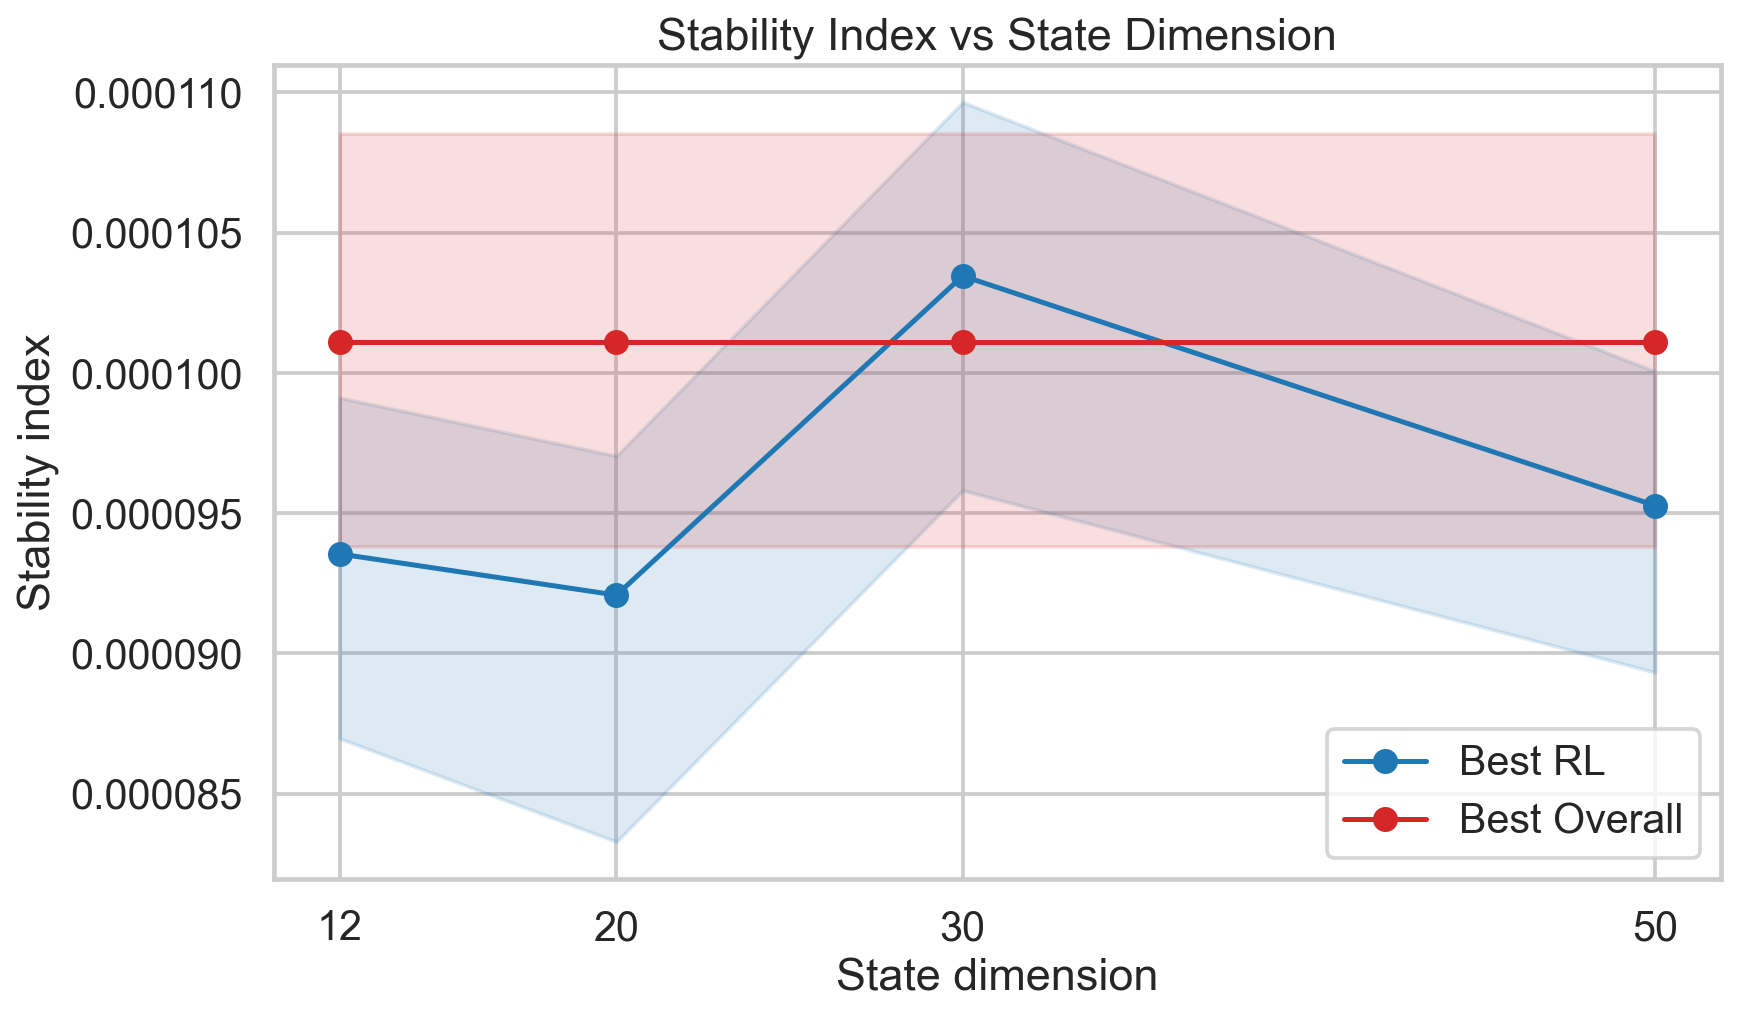
\includegraphics[width=0.82\textwidth]{metric_vs_dimension_stability_index.png}
    \caption{Stability index versus state dimension.}
    \label{fig:en-stability-vs-dim}
\end{figure}

Figures \ref{fig:en-profit-vs-dim}--\ref{fig:en-stability-vs-dim} summarize the same story visually. The best-overall line is flat because the best baseline does not depend on the varying state vector. The best-RL line rises from 12D to 30D on profit, NPV, and reward, then flattens. Default rate improves sharply at 30D, then drifts slightly upward at 50D. Stability changes little, which means the main gain is not a large volatility reduction but a better balance of selectivity, realized performance, and capital usage.

\section{Scenario-Level Results and Interpretation}

\subsection{Why scenario-level analysis is necessary}

The overall leaderboard is informative but incomplete. Because the reward aggregates across six scenarios, it can hide the situations in which RL already matches or exceeds the best non-RL policy and the situations in which it still falls far short. The repository exports scenario-level summaries precisely to avoid that loss of structure.

Two different notions of ``winner'' must be distinguished.
\begin{itemize}[leftmargin=*]
    \item The \emph{reward-based winner} is the controller selected by the repository's official ranking logic.
    \item The \emph{highest-profit winner} is the controller with the largest \texttt{expected\_profit\_mean} in the output tables.
\end{itemize}

These are not always the same controller because the reward function is intentionally multi-objective.

\subsection{Scenario trade-offs in the richest state}

Table \ref{tab:en-scenario-tradeoff-50} focuses on 50D because it is the richest observation design and makes the reward-profit-risk distinction especially visible.

\begin{table}[H]
    \centering
    \small
    \begin{tabular}{p{0.21\textwidth}p{0.20\textwidth}p{0.21\textwidth}p{0.20\textwidth}}
        \toprule
        Scenario                         & Reward-based winner                & Highest-profit winner              & Lowest-default winner     \\
        \midrule
        \texttt{adverse\_stress}         & \texttt{profit\_oriented}          & \texttt{profit\_oriented}          & \texttt{profit\_oriented} \\
        \texttt{base\_market}            & \texttt{dqn}                       & \texttt{dqn}                       & \texttt{dqn}              \\
        \texttt{class\_imbalance\_shift} & \texttt{constraint\_aware\_weekly} & \texttt{constraint\_aware\_weekly} & \texttt{dqn}              \\
        \texttt{drift}                   & \texttt{profit\_oriented}          & \texttt{profit\_oriented}          & \texttt{profit\_oriented} \\
        \texttt{noise}                   & \texttt{profit\_oriented}          & \texttt{risk\_aware\_weekly}       & \texttt{dqn}              \\
        \texttt{split\_policy\_dynamics} & \texttt{profit\_oriented}          & \texttt{profit\_oriented}          & \texttt{dqn}              \\
        \bottomrule
    \end{tabular}
    \caption{Reward-profit-risk leaders in the 50D run, computed from \texttt{outputs/dim\_50/main\_scenario\_summary.csv}.}
    \label{tab:en-scenario-tradeoff-50}
\end{table}

This table shows why the repository cannot be summarized by one sentence such as ``baseline wins'' or ``RL wins.'' The answer depends on the metric and the scenario.

\subsection{Adverse stress}

Adverse stress remains the hardest scenario for RL in every observation size. The reward-based winner is always \texttt{profit\_oriented}, with profit $29{,}336.42$, reward $25{,}150.74$, and default rate $0.1178$. The best RL result is much weaker: in 12D, the best RL controller is \texttt{double\_dqn} with negative profit; in 30D, DQN recovers to a small positive profit of $3{,}413.22$ but still trails the baseline heavily; in 50D, DQN falls back to $-12{,}023.13$.

This pattern is plausible given the scenario design. Adverse stress combines a shock, stronger default pressure, higher noise, and larger loan amounts. Under those conditions, the cost of over-acceptance rises sharply. The myopic-looking \texttt{profit\_oriented} baseline is not actually reckless here because the current-cohort profit preview already reflects much worse cohort economics when the market deteriorates. Its weekly grid search therefore reacts by becoming highly selective, and that conservatism is rewarded.

The cross-week snapshots reinforce the same interpretation. In 30D adverse stress, DQN improves substantially over its 12D and 20D versions, but at week 20 cumulative profit remains only about $7{,}482.68$ compared with \texttt{profit\_oriented}'s $22{,}046.88$. Richer state helps the RL policy survive stress more gracefully, yet it does not close the gap to the best baseline within the current quick-profile budget.

\subsection{Base market}

Base market is where RL looks strongest. In 12D, DQN is already the reward-based winner with profit $86{,}519.38$ and reward $101{,}967.98$. In 20D, Double-DQN becomes the scenario winner and pushes profit to $94{,}321.51$. In 30D, Double-DQN still leads the scenario on reward, while in 50D DQN becomes the clear leader with profit $92{,}105.55$, reward $110{,}521.41$, and default rate $0.1134$.

This result is economically sensible. Base market offers the cleanest environment for representation value to matter. The controller does not have to fight a regime break as severe as adverse stress, so richer state can be used to set a more efficient selective policy. The 50D DQN result is notable because it exceeds the \texttt{profit\_oriented} baseline not only on reward but also on raw profit and default rate. That is the clearest case in the exported results where RL converts richer portfolio state into both higher return and better credit quality.

At the same time, the base-market result should not be over-generalized. The winning RL agent changes across dimensions, and Double-DQN collapses at 50D overall despite once leading this scenario. This again shows that scenario-level success and global robustness are not the same thing.

\subsection{Class-imbalance shift}

Class-imbalance shift is the most consistent win for the conservative rule-based benchmark. The reward-based and profit-based winner is always \texttt{constraint\_aware\_weekly}, with profit $70{,}649.29$ and reward $81{,}420.58$. This makes intuitive sense because the scenario increases the share of lower-quality new applicants. A controller that explicitly internalizes approval, default, and capital penalties has a structural advantage.

The RL story is still important, however. The best RL profit rises from $56{,}746.75$ at 12D to $65{,}715.59$ at 50D, and the lowest default rate in 30D and 50D belongs to DQN rather than to the constraint-aware baseline. This indicates that richer state helps RL recognize composition risk and respond more selectively. What it does not yet do in the quick profile is beat the explicit rule search that is already well aligned with the scenario.

\subsection{Drift}

In the drift scenario, \texttt{profit\_oriented} is the reward-based winner throughout the dimensionality sweep, with profit $59{,}526.10$ and reward $68{,}132.12$. The best RL policy improves from around $40{,}685.98$ in 12D to $52{,}005.69$ in 30D, then softens to $46{,}567.72$ in 50D.

This is a useful counterexample to a naive ``more dimensions always help'' claim. The 30D state, which adds lagged and rolling history, is especially well suited to slow deterioration because drift is a temporal phenomenon. The 50D state adds more descriptors, but those extra coordinates do not improve DQN further in this scenario. The likely implication is that the 30D historical layer captures the essential signal, while the 50D enlargement adds modeling burden without equivalent incremental value.

\subsection{Noise}

The noise scenario reveals the difference between profit maximization and shaped reward most clearly. The highest raw profit belongs to \texttt{risk\_aware\_weekly} at $97{,}377.95$, while the reward-based winner remains \texttt{profit\_oriented} at profit $94{,}589.22$ and reward $112{,}586.40$. In 30D and 50D, DQN achieves lower default rates than both of those baselines and still posts very strong profits, namely $88{,}596.00$ in 30D and $89{,}396.58$ in 50D.

The interpretation is nuanced. Under noisy weekly volumes and measurement disturbance, the risk-aware baseline appears to exploit current profit well, but the reward function still values the more balanced profile produced by \texttt{profit\_oriented}. At the same time, richer-state DQN becomes meaningfully safer, with default rates around $0.1133$ in 30D and $0.1160$ in 50D, compared with \texttt{risk\_aware\_weekly}'s $0.1222$. This is one of the best examples of portfolio-quality trade-off in the current outputs: RL does not win the main ranking, but it creates a more conservative portfolio without collapsing profit.

\subsection{Split-policy dynamics}

The split-policy scenario is designed to reward controllers that can benefit from separate thresholds. The strongest reward-based controller remains \texttt{profit\_oriented} across all dimensions, but the gap to the best RL agent shrinks sharply as state richness increases. The best RL profits are $114{,}185.42$ at 12D, $117{,}912.12$ at 20D, $112{,}439.04$ at 30D, and $119{,}918.57$ at 50D.

The most important observation is not only that 50D DQN reaches almost the same profit as the baseline. It also achieves the lowest default rate in the 50D scenario summary at approximately $0.1093$, compared with \texttt{profit\_oriented}'s $0.1112$. This is exactly the kind of pattern the richer segmented state was meant to uncover: when new and repeat segments evolve in opposite directions, a controller with better segment-specific state can approach baseline-level profitability while becoming slightly safer.

\section{Threshold Behavior and Dynamic Response}

\subsection{What threshold volatility actually shows}

At first glance, the main summaries may suggest that the best RL policies are extremely stable because their reported \texttt{threshold\_volatility\_mean} is exactly zero. That interpretation is correct, but only in a specific sense. Threshold volatility is defined from week-to-week changes within an episode. A value of zero therefore means that the policy keeps the same threshold pair throughout the episode.

The exported weekly logs confirm that this is exactly what happens in the quick-profile winners. For the best RL controller in each dimension, 100\% of evaluation episodes are constant-threshold episodes. The improvement from 12D to 30D does not come from more active week-to-week motion. It comes from selecting better threshold pairs.

\subsection{Episode-static RL winners}

The best RL controllers in the quick profile choose only a small set of episode-level threshold pairs:
\begin{itemize}[leftmargin=*]
    \item 12D DQN selects the pairs $(65,45)$, $(85,35)$, and $(85,50)$ across episodes.
    \item 20D Double-DQN selects $(65,40)$, $(75,50)$, and $(80,55)$.
    \item 30D DQN selects $(70,65)$, $(85,35)$, and $(85,50)$.
    \item 50D DQN selects $(70,45)$, $(85,40)$, and $(85,45)$.
\end{itemize}

This fact is important for honest interpretation. In the active quick-profile experiment, richer state helps the controller identify a better static split policy for the episode more than it induces genuinely adaptive weekly threshold movement. That does not invalidate the dimensionality result. It simply narrows its meaning. The current evidence supports ``better state improves policy quality'' more strongly than ``better state produces richer within-episode adaptation.''

This also helps explain why the leading dynamic baselines still perform so well. Their threshold-volatility means are large---about $9.83$ for \texttt{profit\_oriented} and $9.60$ for \texttt{constraint\_aware\_weekly} in the overall summaries---because they reoptimize or adjust thresholds every week. The quick-profile RL winners, by contrast, are strong mostly as episode-level selectors of static threshold pairs.

\subsection{Early-loss / late-gain diagnostic}

\begin{figure}[H]
    \centering
    
\includegraphics[width=0.82\textwidth]{dim_30/locally_worse_globally_better.png}
    \caption{Diagnostic example of a locally worse but globally better trajectory from the 30D output folder.}
    \label{fig:en-lwgb}
\end{figure}

Figure \ref{fig:en-lwgb} is useful conceptually even though it is only a diagnostic. It illustrates why delayed cash-flow accounting matters for thesis interpretation. A policy can fall behind early because stricter acceptance reduces immediate cohort contribution, then recover strongly once weaker loans that would have defaulted are never originated. That temporal reversal is exactly the type of behavior that a weekly delayed-outcome simulator is designed to capture and that static one-step classification metrics would miss.

\section{Figures for Dimension Comparison}

\begin{figure}[H]
    \centering
    \begin{subfigure}[b]{0.48\textwidth}
        \centering
        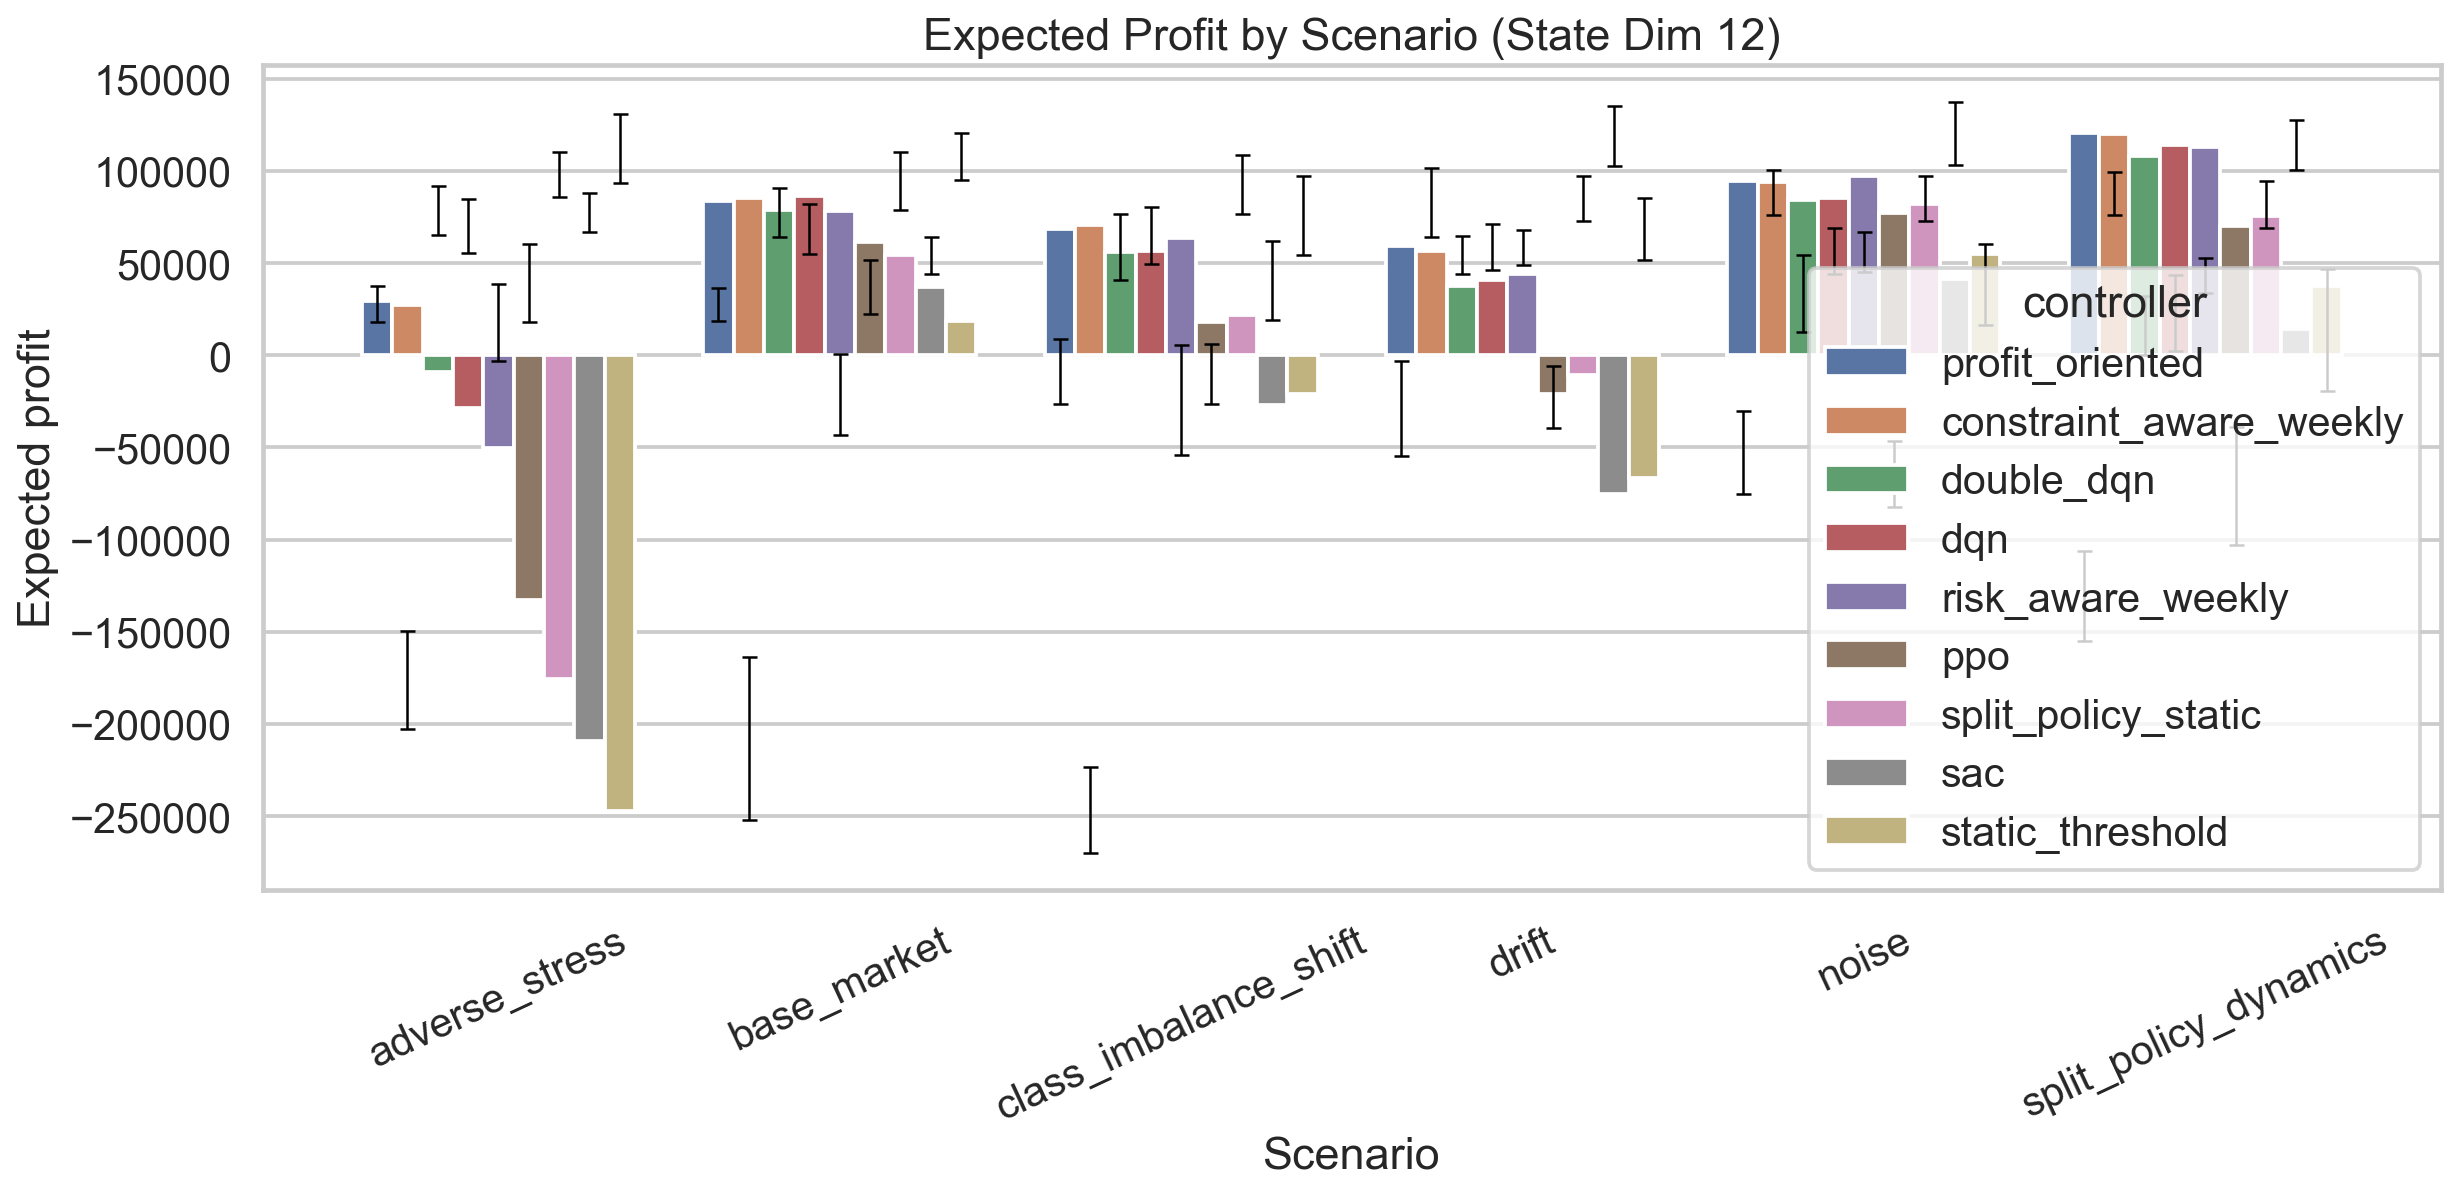
\includegraphics[width=\textwidth]{dim_12/expected_profit_by_scenario_dim12.png}
        \caption{12D}
    \end{subfigure}
    \hfill
    \begin{subfigure}[b]{0.48\textwidth}
        \centering
        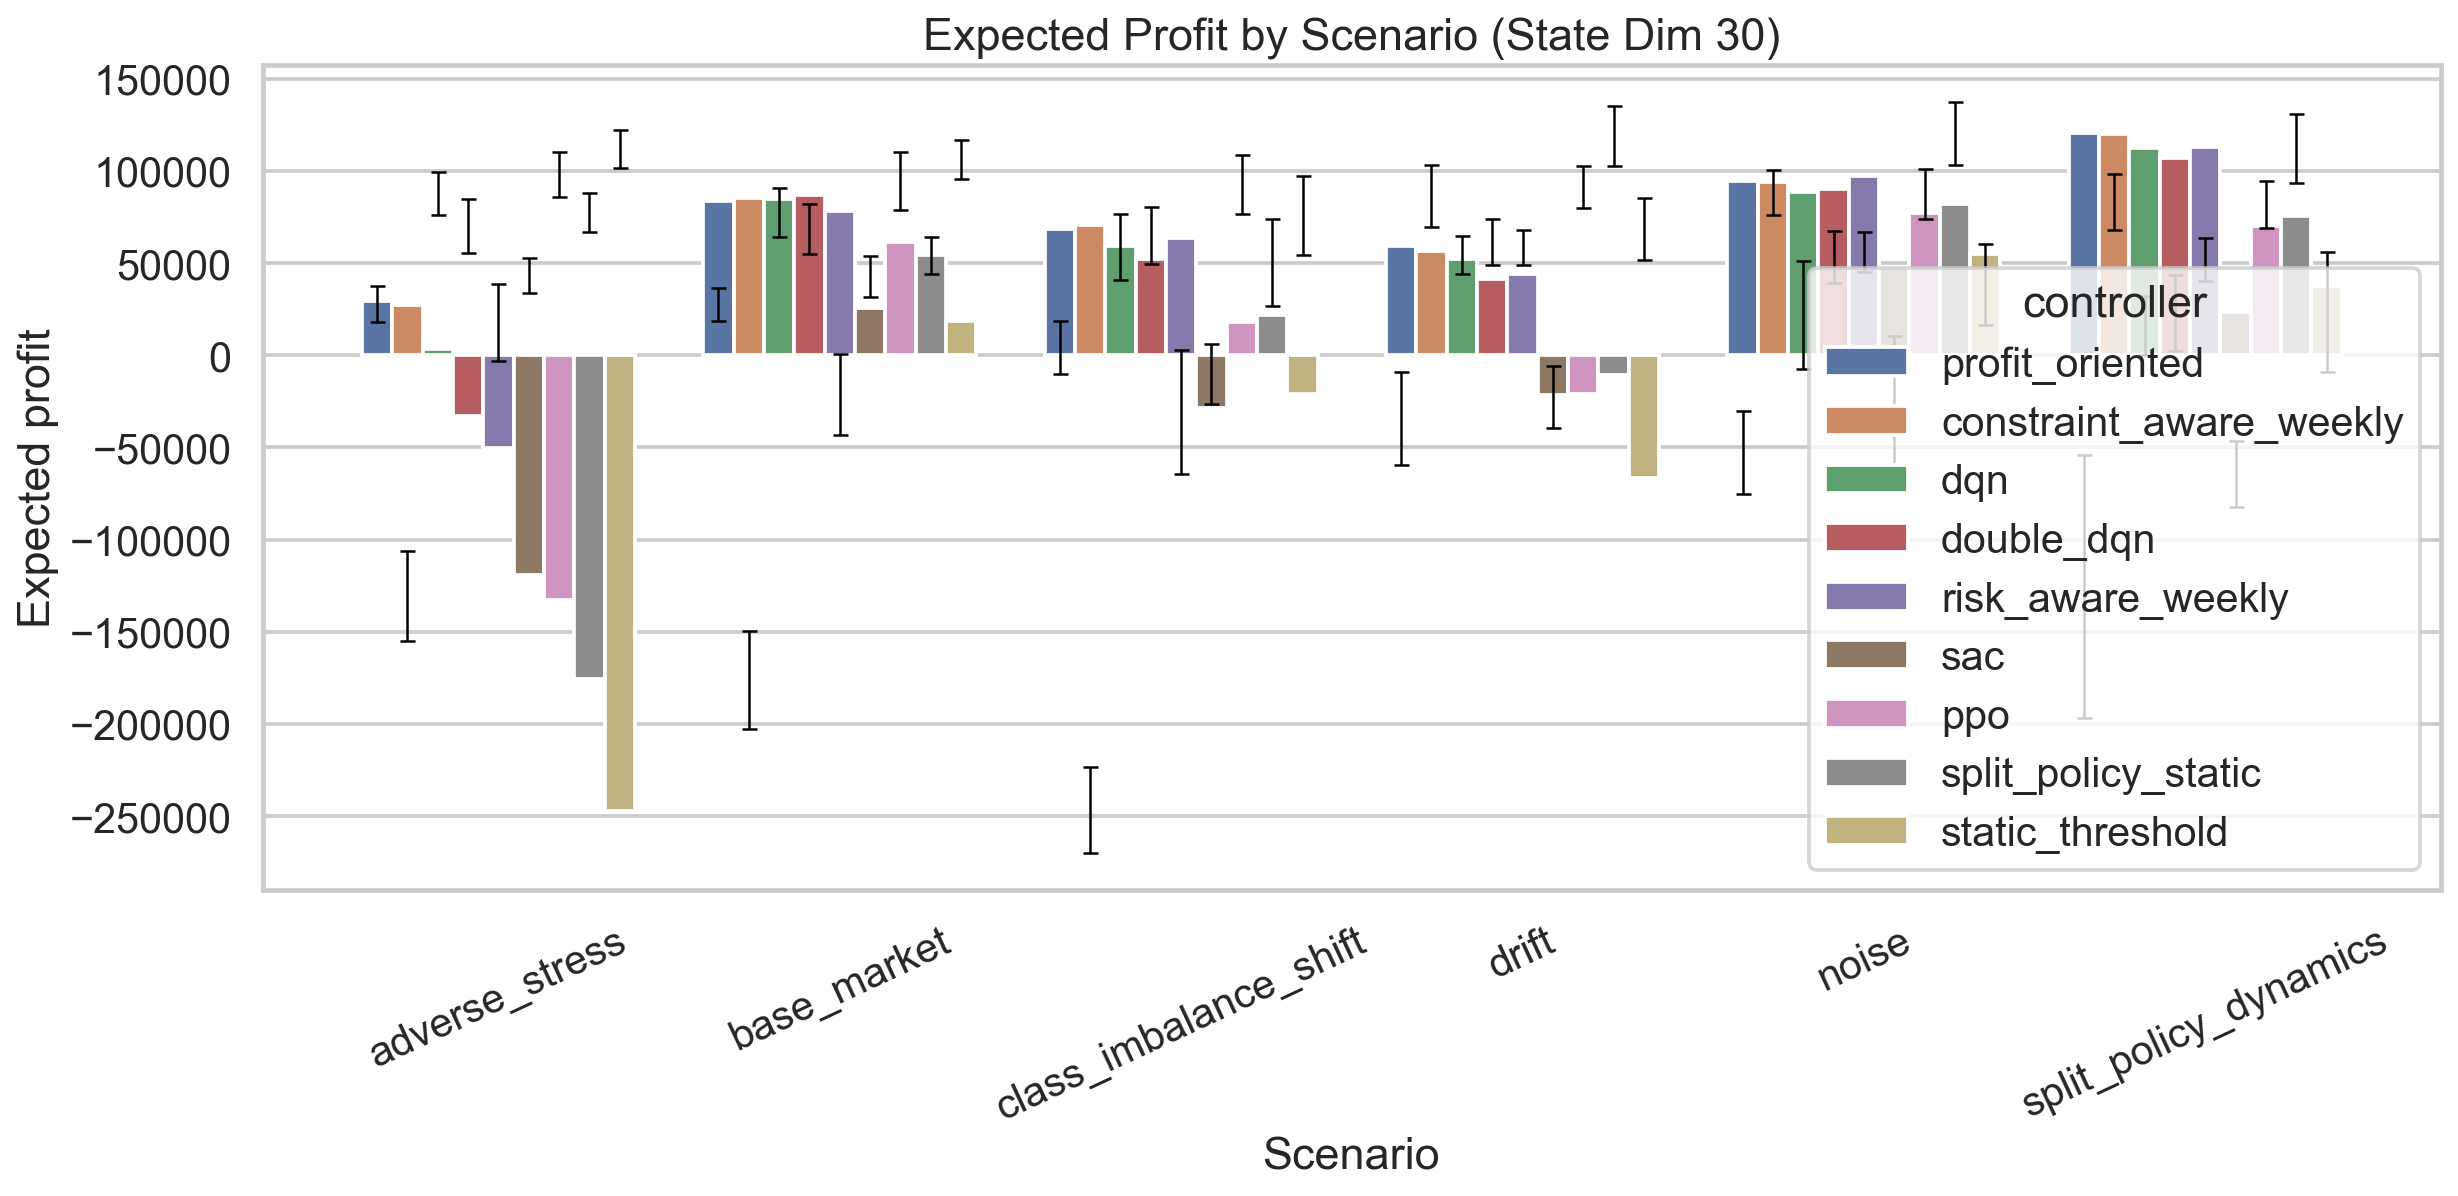
\includegraphics[width=\textwidth]{dim_30/expected_profit_by_scenario_dim30.png}
        \caption{30D}
    \end{subfigure}
    \caption{Scenario-level profit comparison for two representative state sizes.}
    \label{fig:en-scenario-bars-a}
\end{figure}

\begin{figure}[H]
    \centering
    \begin{subfigure}[b]{0.48\textwidth}
        \centering
        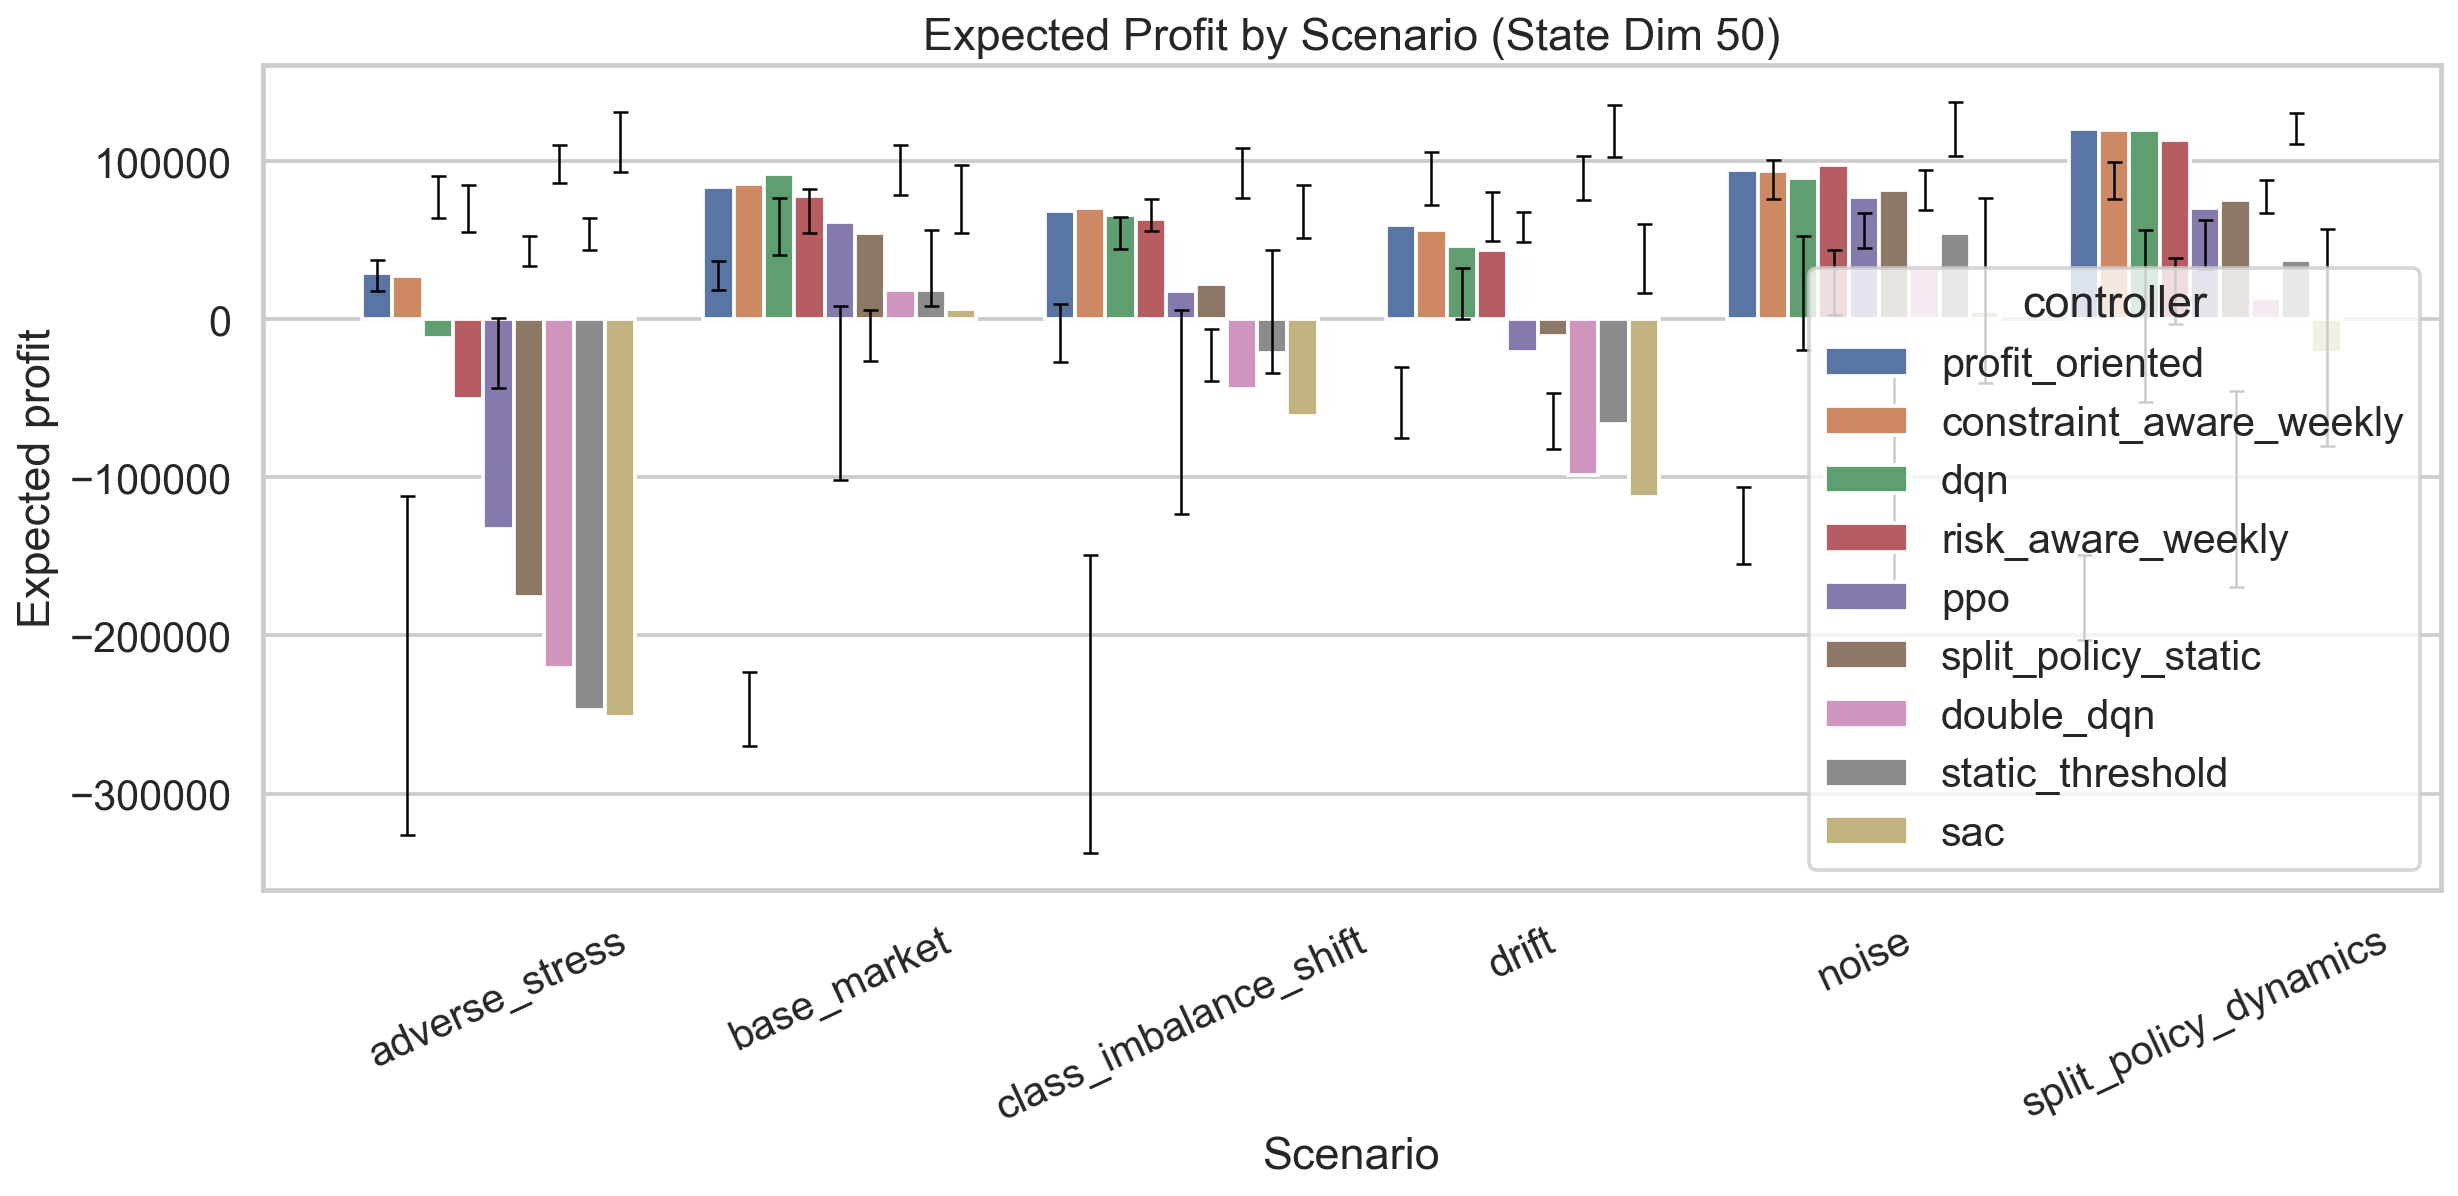
\includegraphics[width=\textwidth]{dim_50/expected_profit_by_scenario_dim50.png}
        \caption{50D}
    \end{subfigure}
    \hfill
    \begin{subfigure}[b]{0.48\textwidth}
        \centering
        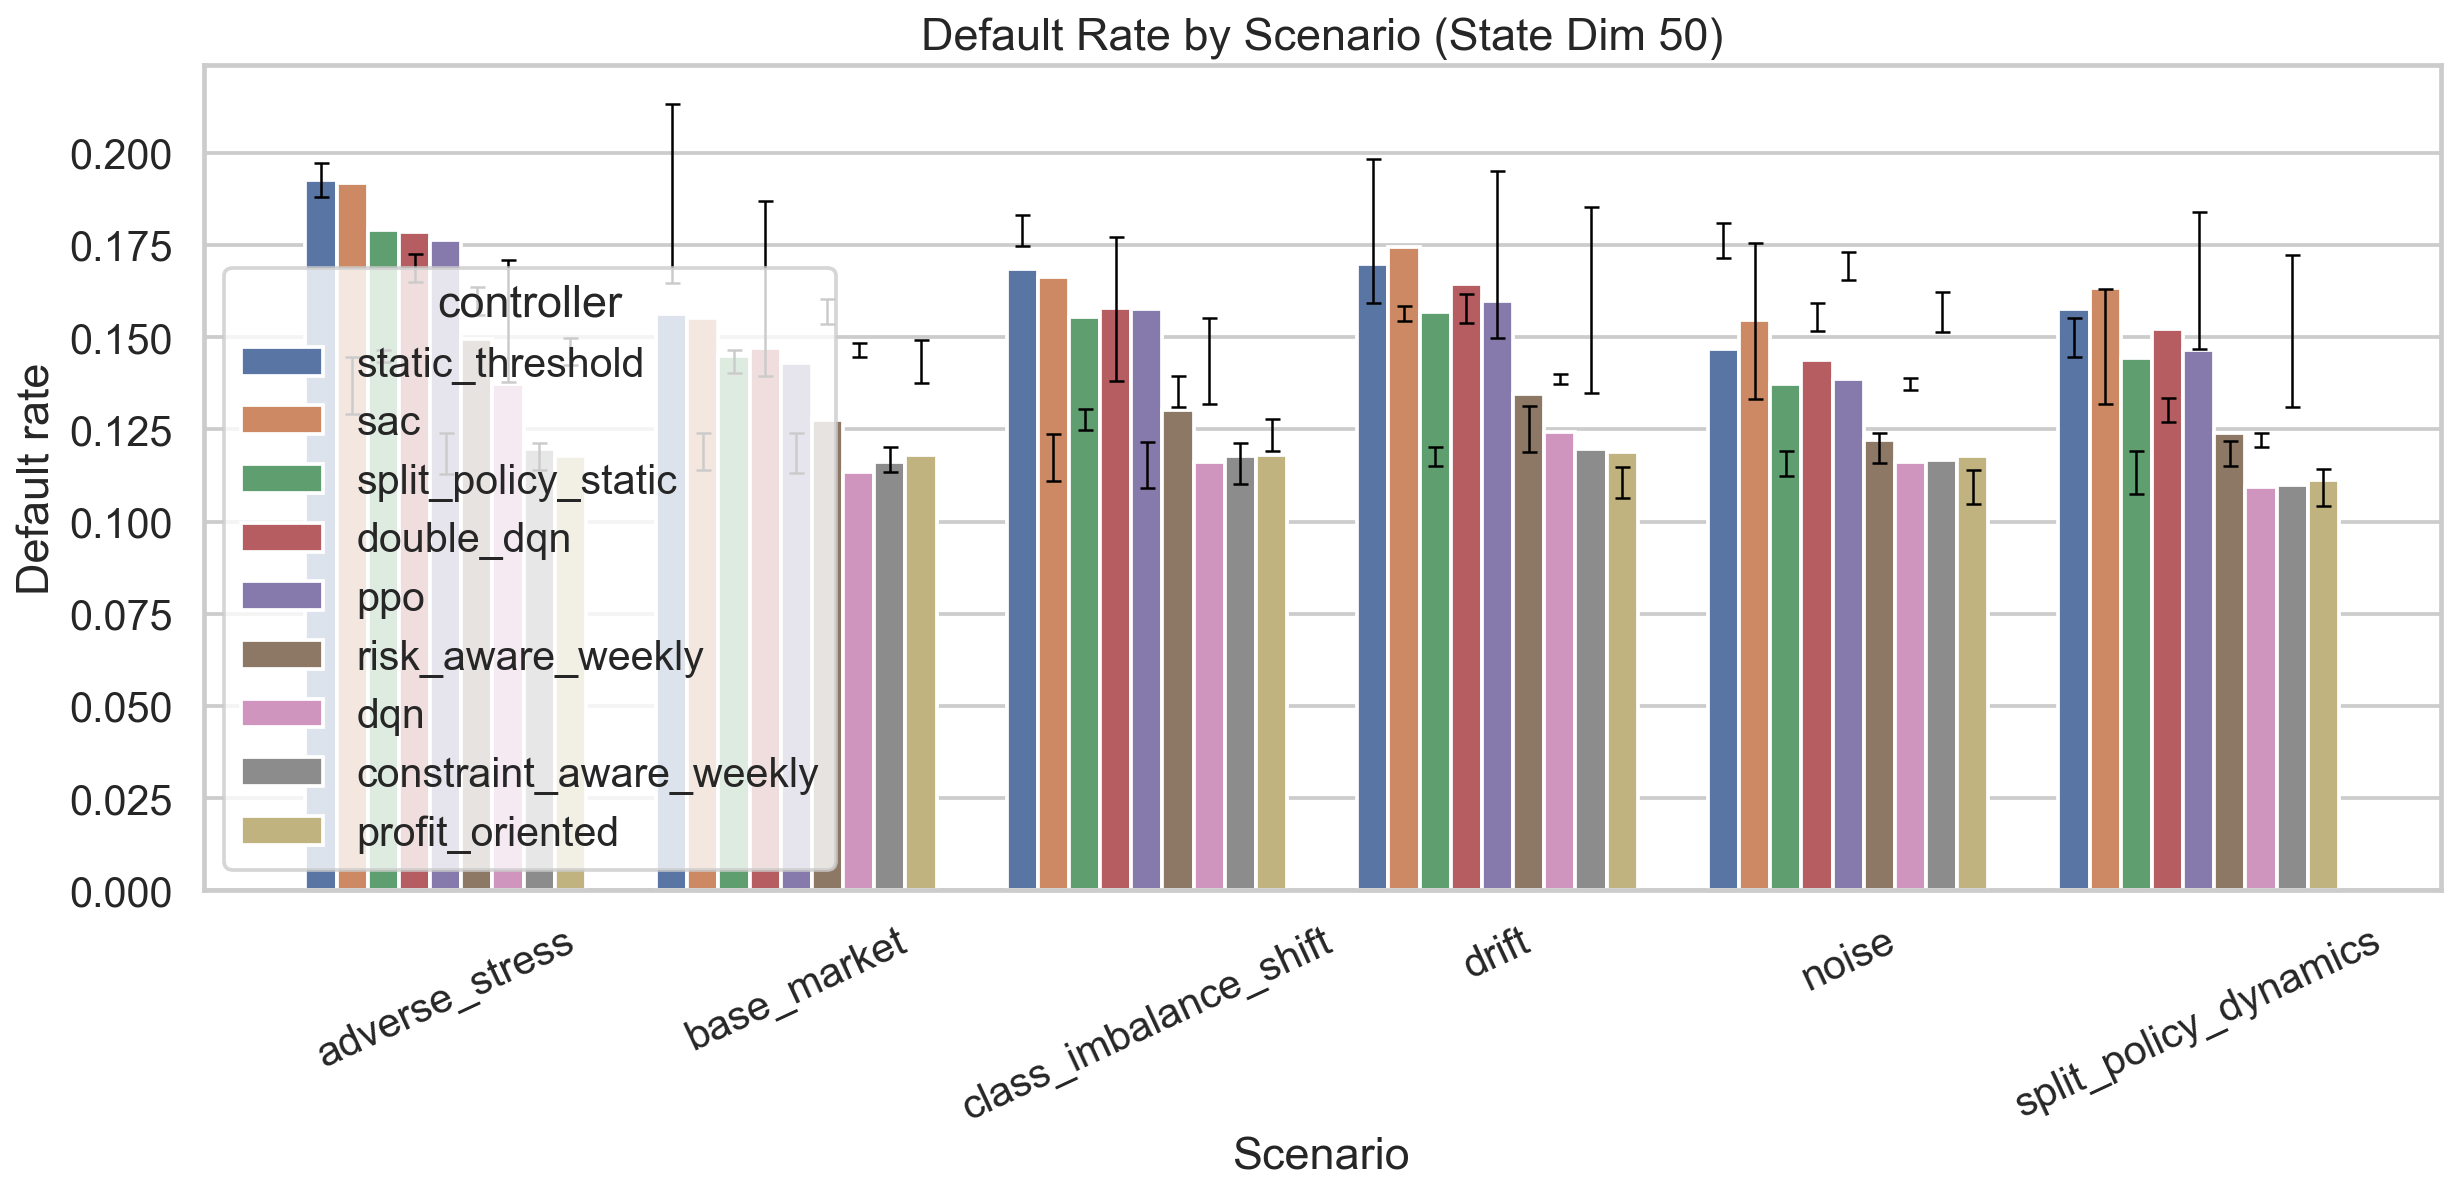
\includegraphics[width=\textwidth]{dim_50/default_rate_by_scenario_dim50.png}
        \caption{50D default-rate comparison}
    \end{subfigure}
    \caption{Rich-state scenario view of profit and default trade-offs.}
    \label{fig:en-scenario-bars-b}
\end{figure}

\begin{figure}[H]
    \centering
    \begin{subfigure}[b]{0.48\textwidth}
        \centering
        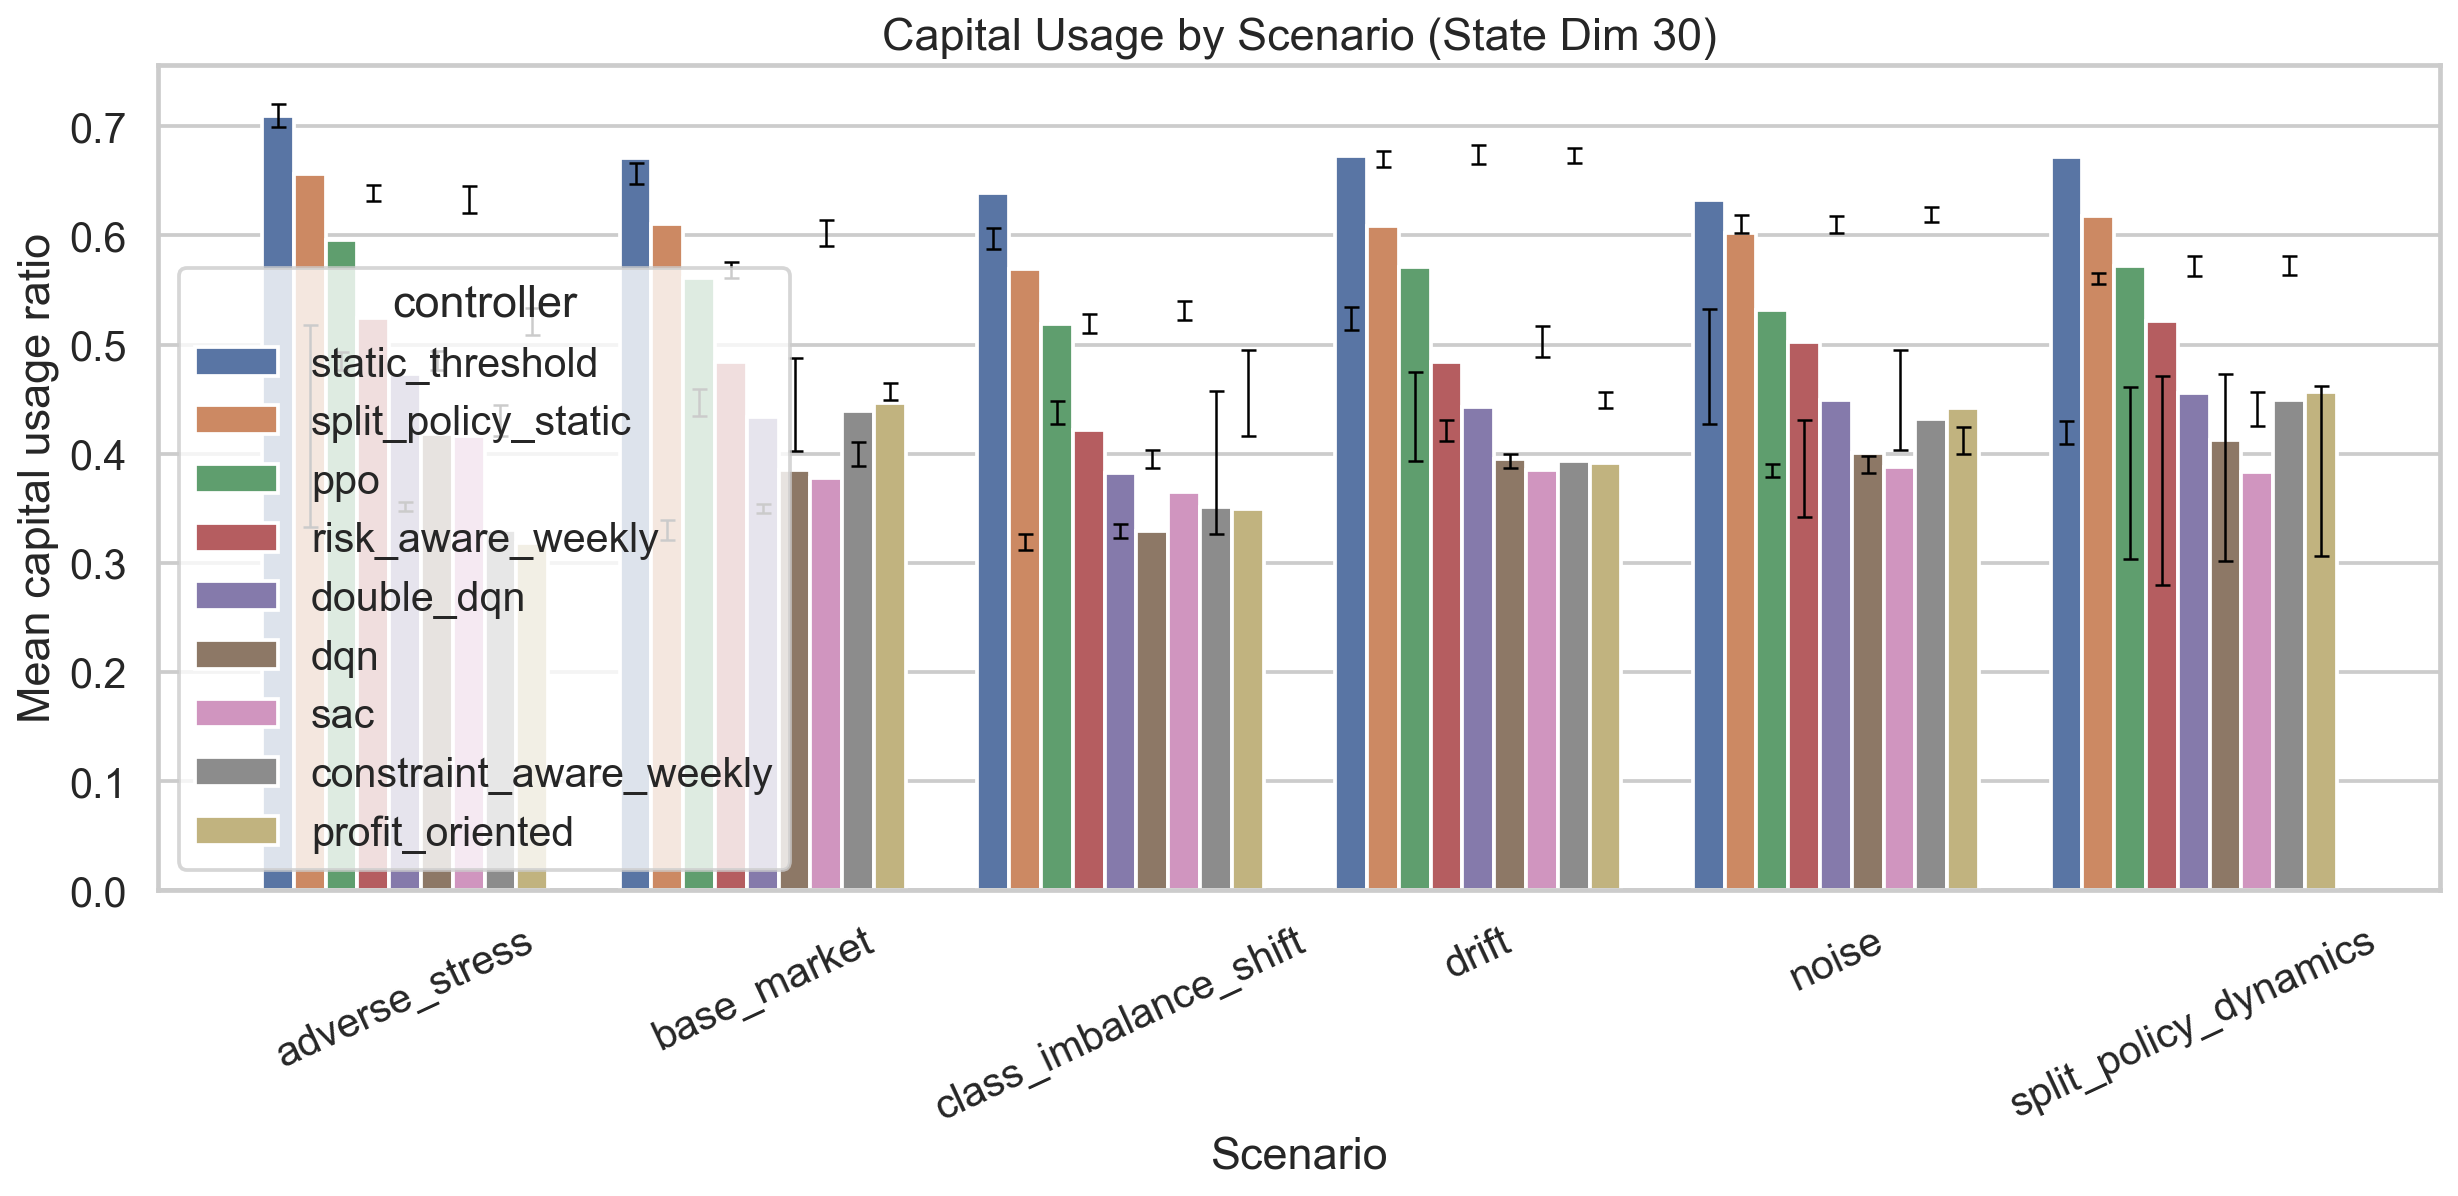
\includegraphics[width=\textwidth]{dim_30/capital_usage_by_scenario_dim30.png}
        \caption{30D capital usage}
    \end{subfigure}
    \hfill
    \begin{subfigure}[b]{0.48\textwidth}
        \centering
        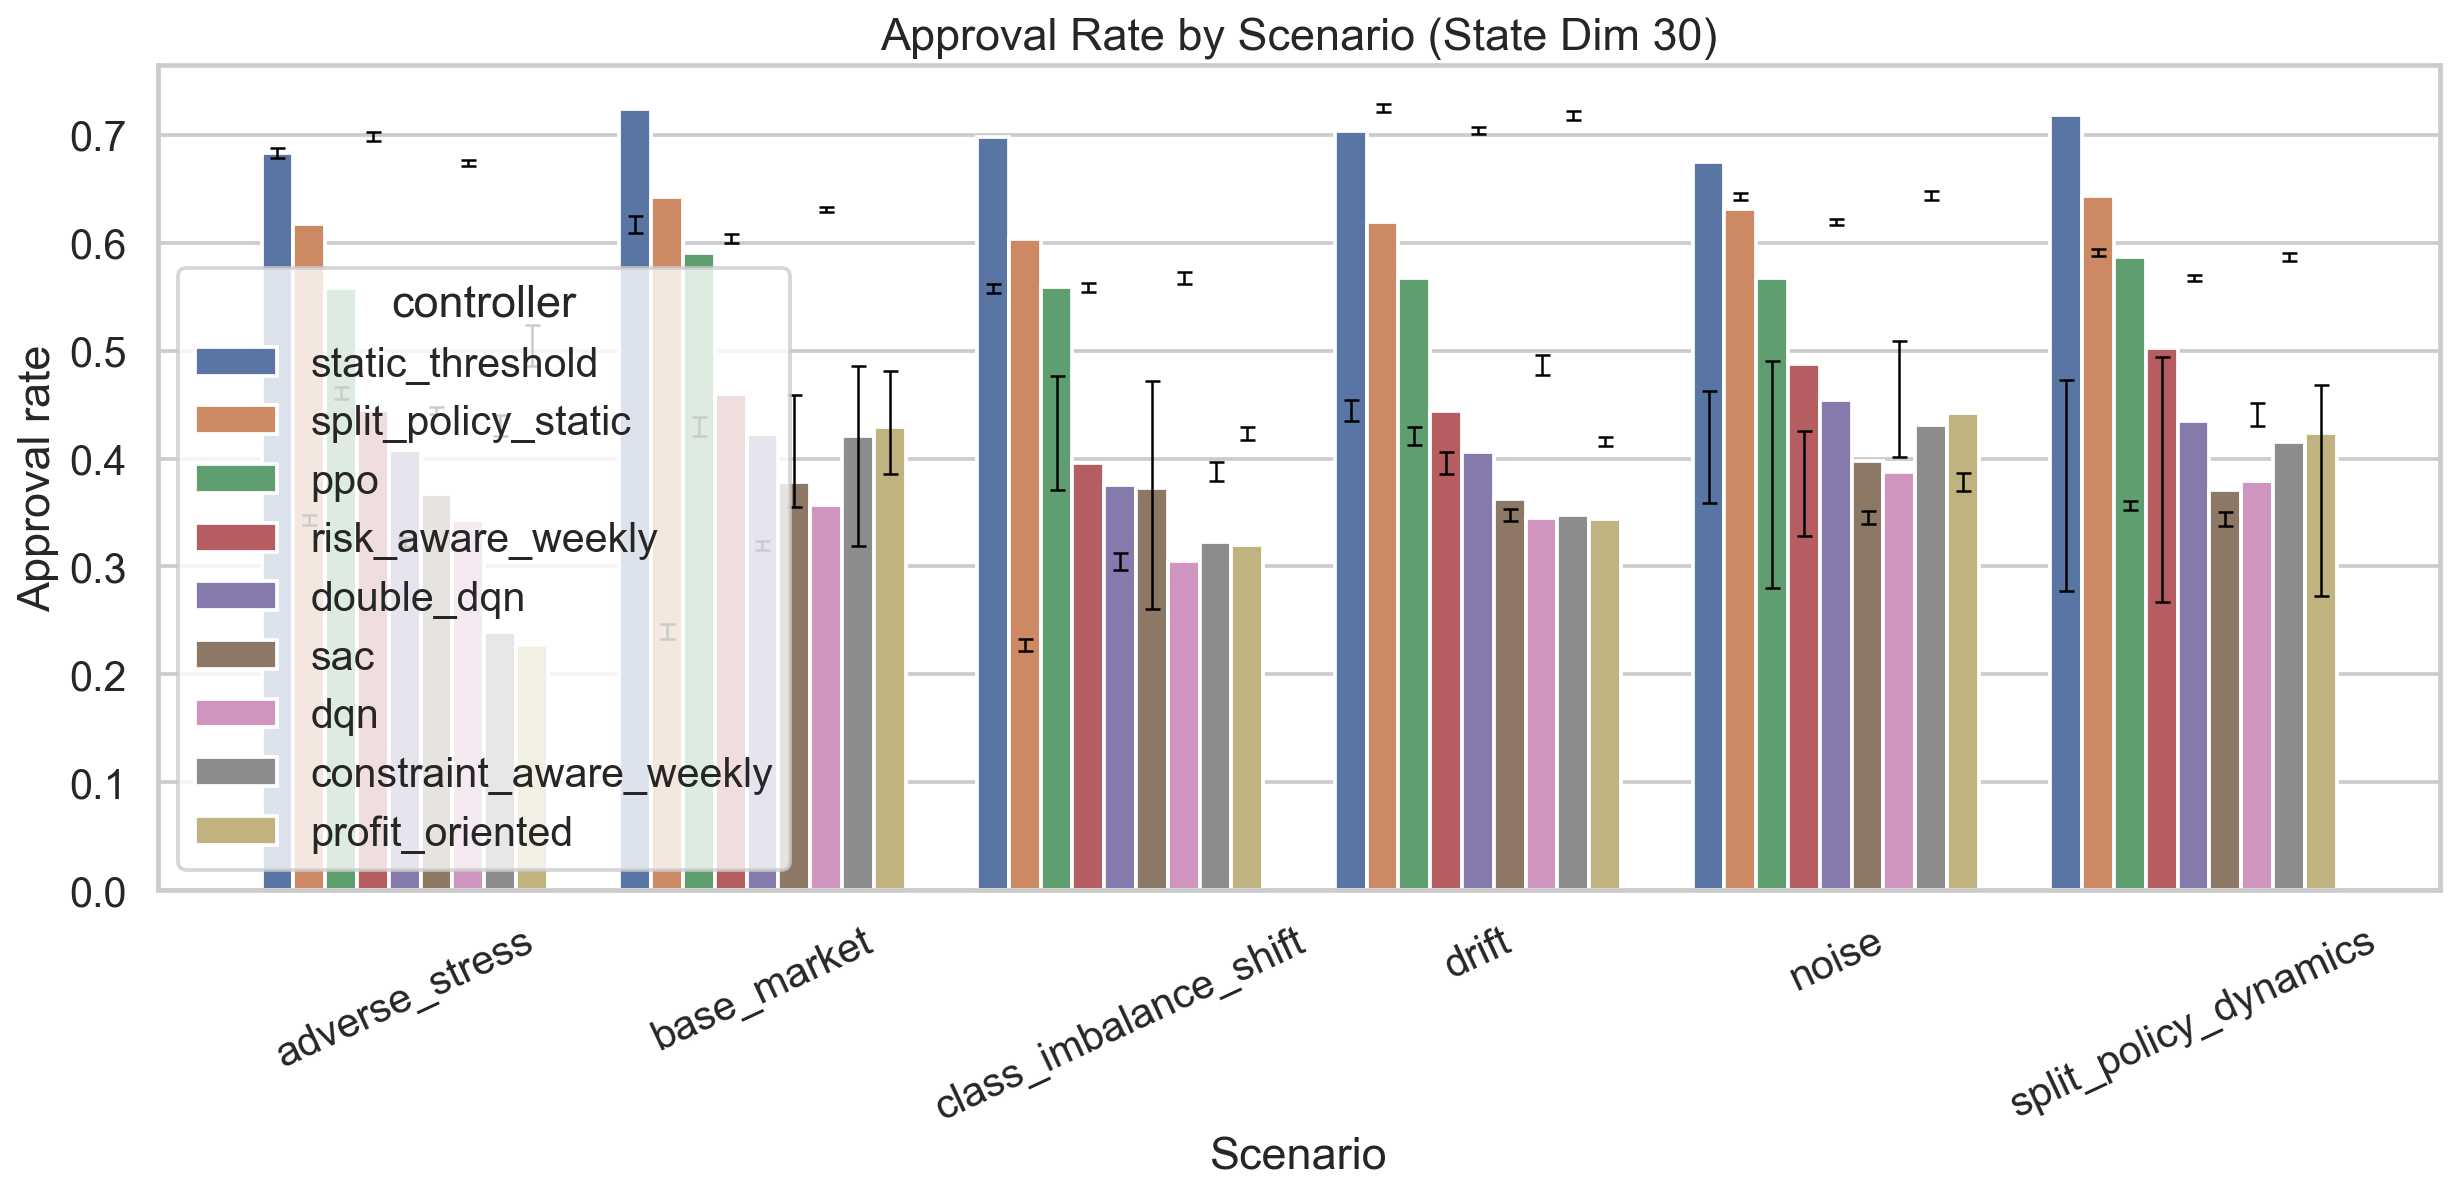
\includegraphics[width=\textwidth]{dim_30/approval_rate_by_scenario_dim30.png}
        \caption{30D approval rate}
    \end{subfigure}
    \caption{Portfolio-allocation trade-offs for the 30D run.}
    \label{fig:en-cap-approval}
\end{figure}

Taken together, Figures \ref{fig:en-scenario-bars-a}--\ref{fig:en-cap-approval} show why the 30D and 50D results are best understood through scenario structure rather than through one scalar curve only. The richest state does help in several places, especially \texttt{base\_market}, \texttt{class\_imbalance\_shift}, and \texttt{split\_policy\_dynamics}, but it does not remove the RL deficit under \texttt{adverse\_stress} and does not overturn the dominance of conservative rule-based search in \texttt{drift}.

\section{Discussion}

\subsection{Why 30D is the most balanced state size}

The 30D state is the strongest compromise in the current outputs. It delivers the largest jump in best-RL reward, improves profit and NPV materially, lowers default rate relative to 20D, and does so with lower approval and capital usage. In other words, it improves the quality of selectivity rather than only the quantity of lending.

The extra information added between 20D and 30D is not arbitrary. It is precisely the historical memory layer: lagged approval, lagged realized default, lagged realized profit, lagged capital usage, rolling means, rolling profit variability, and lagged threshold changes. Those variables are well matched to a weekly control problem because they tell the controller whether the latest week is exceptional or part of an emerging pattern. That is especially useful in drift, noise, and composition-shift environments.

\subsection{Why 50D saturates}

The move from 30D to 50D still adds meaningful descriptors, but their incremental value is smaller. Segment-level means, rolling reward moments, cumulative totals to date, and threshold-gap history make the observation richer, yet the best RL reward no longer improves. In practice, this looks like a saturation frontier: once the controller already knows current performance, recent history, and lagged threshold behavior, the additional segmentation and stability coordinates do not produce a comparable gain in decision quality under the current training budget.

There is also a more cautionary reading. The 50D run is not merely ``no better.'' It actively harms some algorithms. Double-DQN falls from a positive reward of $69{,}812.02$ at 20D to $-79{,}329.16$ at 50D, and SAC deteriorates sharply as well. This means that the 50D state can be viewed as both richer and more optimization-demanding. The state itself is not bad, but its control value is conditional on the learning algorithm and the training budget.

\subsection{Why the best baseline still wins overall}

The persistent dominance of \texttt{profit\_oriented} and \texttt{constraint\_aware\_weekly} is not accidental. Both baselines exploit privileged structural alignment with the environment.
\begin{itemize}[leftmargin=*]
    \item They perform explicit weekly search over the same threshold grid that the environment exposes.
    \item They do not have to learn a value function or policy representation from limited episodes.
    \item Their decisions are directly tied to the simulator's current weekly economics and constraint structure.
\end{itemize}

Under the quick profile, RL has only 12 training episodes per seed, which is deliberately small. The fair interpretation is therefore not ``RL failed.'' The fair interpretation is that strong hand-crafted policy search remains extremely competitive in a well-structured simulator, while RL becomes meaningfully better when the state is informative enough and the scenario is favorable enough.

\subsection{Portfolio-quality trade-offs}

The dimensionality experiment is most interesting where several metrics move in opposite directions. The best RL controller at 20D increases approval rate and capital usage relative to 12D, but also slightly worsens default rate. The 30D controller reverses that pattern: it becomes more selective, uses less capital, and improves reward strongly. The 50D controller then relaxes again, with higher approval and capital usage but nearly flat reward.

This sequence is exactly the kind of portfolio trade-off that a thesis should emphasize. Better results do not always mean ``approve more'' or ``reduce default'' in isolation. What matters is the joint movement of profit, default, capital usage, and stability. The 30D result is strong because the joint movement is favorable. The 50D result is weaker because the additional approval and capital consumption do not translate into additional reward.

\subsection{What the current results do and do not prove}

The current evidence does prove several things.
\begin{itemize}[leftmargin=*]
    \item State design matters materially for RL quality.
    \item The marginal value of additional state information is non-linear.
    \item Richer state can improve profitability while preserving or even improving risk metrics in some scenarios.
    \item The benefit of richer state is algorithm-dependent.
\end{itemize}

It does \emph{not} prove that 50D is universally too large, that 30D would remain optimal under a much larger training budget, or that RL is incapable of learning genuinely dynamic weekly policies. Those stronger claims would require a longer-horizon training study, not only the current quick-profile outputs.

\section{Limitations}

Several limitations should be stated directly.
\begin{itemize}[leftmargin=*]
    \item The simulator is synthetic. Its segment parameters and scenarios are economically plausible, but they are not calibrated to confidential production portfolios.
    \item The quick profile is intentionally small. Twelve training episodes per seed are sufficient for an end-to-end controlled experiment, not for a final convergence claim.
    \item The reward is a designed objective, not a discovered one. The relative ranking of controllers is therefore partly a function of the chosen trade-off between profitability, approval pressure, capital usage, and volatility.
    \item The exported confidence intervals quantify uncertainty inside the simulation generator. They do not, by themselves, establish external validity on real bank data.
    \item The best RL policies in this profile are episode-static threshold pairs. Therefore, the current evidence for adaptive weekly threshold movement is weaker than the evidence for better episode-level threshold selection.
\end{itemize}

These limitations do not weaken the core methodological contribution. They simply define the correct boundary of the claim.

\section{Novelty and Contribution}

The novelty of the study lies less in inventing a brand-new RL algorithm and more in combining several research ingredients in one controlled experimental design.
\begin{itemize}[leftmargin=*]
    \item The project formulates credit-scoring control as weekly portfolio threshold management rather than one-shot application classification.
    \item It makes delayed outcomes first-class objects of the environment, including late recovery and terminal settlement.
    \item It models new and repeat applicants separately and allows simultaneous control of both thresholds.
    \item It evaluates learned policies against a diverse and economically interpretable baseline set.
    \item It turns state design itself into a controlled research variable and documents the resulting saturation effect.
\end{itemize}

This is why the thesis contribution should be described as a contribution in \emph{problem formulation, simulation design, and experimental methodology}, not only as a leaderboard comparison.

\section{Conclusion}

The current repository supports a clear and evidence-based conclusion. Increasing observation dimensionality from 12 to 20 and then to 30 features improves the best RL frontier substantially. The largest gain occurs at 30D, where DQN reaches profit $66{,}758.29$, NPV $64{,}755.07$, cumulative reward $78{,}219.69$, and a reduced default rate of $0.1185$ with lower approval and capital usage than the 20D winner. Moving from 30D to 50D adds almost no additional reward and slightly weakens the portfolio balance, which is the signature of saturation.

At the same time, the thesis should not compress the results into a simplistic RL-versus-baseline slogan. The strongest overall controller remains the rule-based \texttt{profit\_oriented} baseline, with \texttt{constraint\_aware\_weekly} essentially tied behind it. RL is already competitive and occasionally dominant in some scenarios, especially stable or richly segmented ones, but it is not yet the universal winner under the current quick-profile budget.

The most defensible final statement is therefore the following. In this weekly delayed-outcome credit-scoring simulator, state representation is a first-order determinant of RL quality. Richer state adds real control value up to an intermediate regime, especially once lagged and rolling portfolio history are incorporated. Beyond that point, the marginal gain flattens and can even reverse for some algorithms. For the exported quick-profile results, 30D is the most balanced RL state design, 50D demonstrates diminishing returns, and strong rule-based baselines remain the benchmark that RL must still surpass more consistently.

\end{document}
